% Cheyne Homberger - GMA talk 2014 - cheyne.homberger@gmail.com

\documentclass[xcolor=dvipsnames]{beamer}
  % \includeonlyframes{current}

  % \usetheme[]{Hannover}
  % \usetheme{Warsaw}
  \usecolortheme[named=teal]{structure}
  \setbeamerfont{frametitle}{size = {\large}, family=\rmfamily}
  \setbeamertemplate{navigation symbols}{}
  % to make a handout, uncomment these
  % \usepackage{pgfpages}
  % \pgfpagesuselayout{8 on 1}

  % packages for extra math symbols
  \usepackage{amsthm, amsmath, amssymb} 

  % I like these fonts better
  \usepackage{mathpazo}
  % \usepackage{palatino, mathpazo} 
  % \renewcommand{\familydefault}{\rmdefault}

  % lets you draw nice pictures
  \usepackage{tikz}

  \definecolor{lg}{rgb}{.85,.85,.85}
  \DeclareMathOperator{\Av}{Av}

  \newcommand{\Avn}{\Av_n(123)}
  \newcommand{\Avns}{\Av_n^*(123)}

  \newcommand{\num}{f}
  \newcommand{\ds}{\displaystyle}
  \newcommand{\ra}{\rightarrow}
  \newcommand{\R}{\mathbb{R}}
  \newcommand{\si}{\sigma}
  \renewcommand{\S}{\mathfrak{S}}

  \newcommand{\Ex}[1]{\mathbb{E}\left[ #1 \right]}

  \addtolength{\headheight}{-12pt}
  \addtolength{\textheight}{12pt}

% abstract: 
% Permutations are a fundamental object across all areas of mathematics, and
% their wide variety of equivalent definitions endows them with a rich and
% complex structure.  By viewing smaller permutations as patterns within larger
% ones, the set of all permutations becomes a partially ordered set which has
% become a major topic of research in the last half-century.  Starting with a
% an overview of the area, this talk provides an accessible introduction to the
% area of permutation patterns (with plenty of pictures and some hand-waving).
% In particular, we explore several longstanding conjectures, some recently
% opened questions, and a new result on patterns within random permutations. 


% ===================================================================== %
\begin{document}
\title[Patterns in Permutations]%
  {\rmfamily \Large Patterns Within Random Permutations \\
  \normalsize Some Open (and Recently Closed) Questions}

\author{Cheyne Homberger}
\date{\today}

\begin{frame}
  \titlepage
\end{frame}

\section{Introduction}
\subsection{}


% =========================================================================== %
\begin{frame} \frametitle{Permutations: Representation/Notation}
  \begin{block}{Definition}
    An $n$-\emph{permutation} is a bijection $p:[n] \ra [n]$. \\
    The set of all $n$-permutations is denoted by $\S_n$. 
  \end{block}

  \vspace{1pc}

    
  \begin{center}
  \begin{block}{Two/One-Line Notation}
  \begin{tikzpicture}[scale=1.4]
    \foreach \p [count=\i] in {3,5,1,4,2}{
      \node at (\i,1) {\i};
      \node at (\i,0) {\p};
      \draw[->] (\i, .65) -> (\i, .35); }
  \end{tikzpicture}
  \end{block}
  \end{center}


\end{frame}


\begin{frame} \frametitle{Plotting Permutations}

  \begin{block}{Definition}
    If $\pi = \pi_1 \pi_2 \cdots \pi_n$ is a permutation written in one line
    notation, then the \emph{plot} of $\pi$ is the set of points 
    $$ \{ (1, \pi_1), (2, \pi_2), \cdots (n, \pi_n) \} \subset \mathbb{R}^2 $$
  \end{block}

  \pause 
  \begin{center}
  \begin{tikzpicture}[scale = .5,
                      dot/.style={circle, fill=teal, inner sep=.5mm}]
    \foreach \y [count = \x] in {3,5,1,4,2}
    \node[dot] at (\x,\y) {};
  \end{tikzpicture}
  \end{center}
  $$ \pi = 35142 $$

\end{frame}



% =========================================================================== %
\begin{frame} \frametitle{Dots on a Plane} 
  \only<1->{
  \begin{block}{Definition} 
    Let $A$ and $B$ be two sets of $n$ points in $\R^2$, each with the property
    that no two points lie on the same horizontal or vertical line. \\
    Say that $A \sim B$ if $A$ can be transformed into $B$ by stretching, 
    contracting, and translating the axes horizontally and vertically.
  \end{block}
  }
  
  \vspace{.5pc}

  \pause 

  \begin{block}{Example}
    \vspace{1pc}
    \begin{tikzpicture}[scale = .5,
                        every node/.style={circle, fill=teal, inner sep=.5mm}]
      \node at (1,3.5) {};
      \node at (1.3,4.5) {};
      \node at (3,.5) {};
      \node at (3.4,4) {};
      \node at (5,1) {};
    \end{tikzpicture}
    \hspace{1pc}
    \raisebox{2.5pc}{$\sim$}
    \hspace{1pc}
    \begin{tikzpicture}[scale = .5,
                        every node/.style={circle, fill=teal, inner sep=.5mm}]
      \node at (1,2) {};
      \node at (2.5,5) {};
      \node at (3,1) {};
      \node at (3.5,4) {};
      \node at (5,1.5) {};
    \end{tikzpicture}
    \hspace{1pc}
    \pause
    \raisebox{2.5pc}{$\sim$}
    \hspace{1pc}
    \begin{tikzpicture}[scale = .5,
                        dot/.style={circle, fill=teal, inner sep=.5mm}]
      \foreach \y [count = \x] in {3,5,1,4,2}
      \node[dot] at (\x,\y) {};
    \end{tikzpicture}

    \pause
    \vspace{1pc}
    { \hfill $\pi = 35142$ \hspace{3pc}}
  \end{block}
\end{frame}


% =========================================================================== %
\begin{frame} \frametitle{Permutation Patterns} \pause
  \begin{block}{Definition}
    Let $\pi = \pi_1 \pi_2 \cdots \pi_n$ and 
    $\si = \si_1 \si_2 \cdots \si_k$ be two permutations written in one-line
    notation. $\pi$ \emph{contains $\si$ as a pattern} (written $\si \prec
    \pi$) if there is some subsequence $\pi_{i_1} \pi_{i_2} \ldots \pi_{i_k}$
    which is in the same relative order as the entries of $\si$ (i.e.,
    $\pi_{i_j} < \pi_{i_k}$ if and only if $\si_j < \si_k$).  
  \end{block}
  \pause 

  \vspace{1pc}

  \begin{tikzpicture}[scale = .5,
                      dot/.style={circle, fill=teal, inner sep=.5mm}]
    \foreach \y [count = \x] in {3,5,1,4,2}
    \node[dot] at (\x,\y) {};
  \end{tikzpicture}
  %
    \hspace{1pc}
    \raisebox{2pc}{$=$}
    \hspace{1pc}
  %
  \begin{tikzpicture}[scale = .5,
                      dot/.style={circle, fill=teal, inner sep=.5mm}]
    \node[dot] at (1,3) {};
    \node[dot, fill = lg] at (2,5) {};
    \node[dot] at (3,1) {};
    \node[dot] at (4,4) {};
    \node[dot, fill = lg] at (5,2) {};
  \end{tikzpicture}
  %
    \hspace{1pc}
    \raisebox{2pc}{$\succ$}
    \hspace{1pc}
  %
  \begin{tikzpicture}[scale = .5,
                      dot/.style={circle, fill=teal, inner sep=.5mm}]
    \node[dot] at (1,3) {};
    \node[dot, fill=white] at (2,5) {};
    \node[dot] at (3,1) {};
    \node[dot] at (4,4) {};
    \node[dot, fill=white] at (5,2) {};
  \end{tikzpicture}

  \vspace{1pc}

  $$ 35142 \qquad \succ \qquad 213 $$


\end{frame}


\newgeometry{margin=0mm}
\begin{frame} \frametitle{\hspace{28pt}The Pattern Poset} \pause
  \begin{center}
    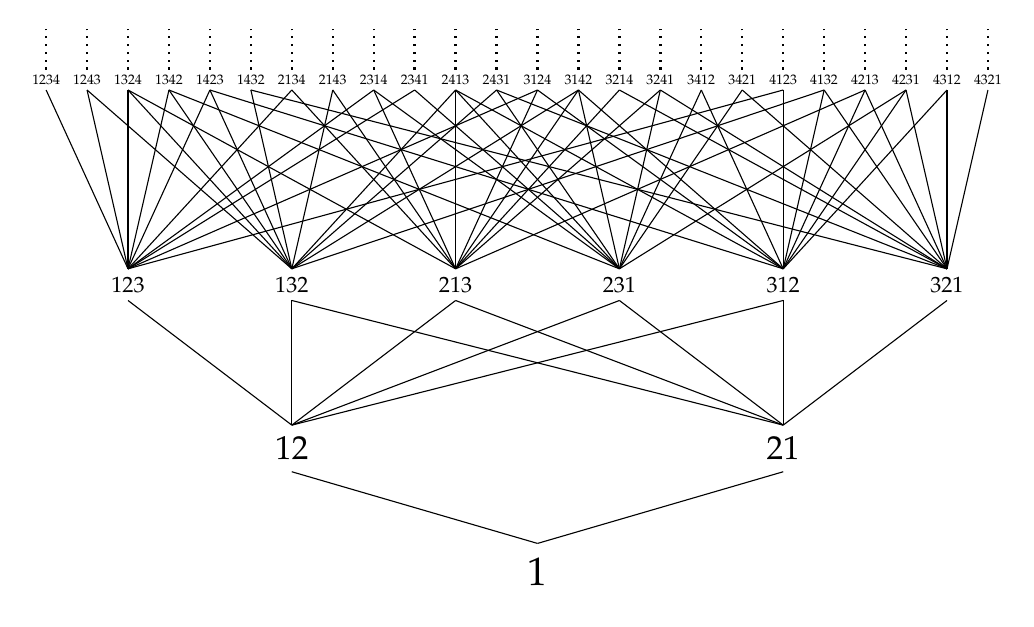
\begin{tikzpicture}[
    every node/.style={},
    scale=.52]
      {\Large
      \node (1) at (12,0) {1};
      }

      \pause

      {\large
      \node (12) at (6,3) {12};
      \node (21) at (18,3) {21};
      }

      \pause

      \draw (12.south)-- (1.north);
      \draw (21.south) -- (1.north);

      \pause

      {\footnotesize
      \node (123) at (2 ,7) {123};
      \node (132) at (6 ,7) {132};
      \node (213) at (10,7) {213};
      \node (231) at (14,7) {231};
      \node (312) at (18,7) {312};
      \node (321) at (22,7) {321};
      }

      \pause

      \draw (123.south) -- (12.north);
      \draw (132.south) -- (12.north);
      \draw (213.south) -- (12.north);
      \draw (231.south) -- (12.north);
      \draw (312.south) -- (12.north);
      
      \draw (132.south) -- (21.north);
      \draw (213.south) -- (21.north);
      \draw (231.south) -- (21.north);
      \draw (312.south) -- (21.north);
      \draw (321.south) -- (21.north);

      \pause
      
      {\tiny
      \node (1234) at (0 ,12) {1234};
      \node (1243) at (1 ,12) {1243};
      \node (1324) at (2 ,12) {1324};
      \node (1342) at (3 ,12) {1342};
      \node (1423) at (4 ,12) {1423};
      \node (1432) at (5 ,12) {1432};

      \node (2134) at (6 ,12) {2134};
      \node (2143) at (7 ,12) {2143};
      \node (2314) at (8 ,12) {2314};
      \node (2341) at (9 ,12) {2341};
      \node (2413) at (10,12) {2413};
      \node (2431) at (11,12) {2431};

      \node (3124) at (12,12) {3124};
      \node (3142) at (13,12) {3142};
      \node (3214) at (14,12) {3214};
      \node (3241) at (15,12) {3241};
      \node (3412) at (16,12) {3412};
      \node (3421) at (17,12) {3421};

      \node (4123) at (18,12) {4123};
      \node (4132) at (19,12) {4132};
      \node (4213) at (20,12) {4213};
      \node (4231) at (21,12) {4231};
      \node (4312) at (22,12) {4312};
      \node (4321) at (23,12) {4321};
      }

      \pause 

      % 123
      \foreach \p in {1234, 1243, 1324, 1342, 1423, 2134, 2314, 2341, 3124, 4123}
        \draw (\p.south) -- (123.north);
      % 132
      \foreach \p in {1243, 1324, 1342, 1423, 1432, 2143, 2413, 2431, 3142, 4132}
        \draw (\p.south) -- (132.north);
      % 213
      \foreach \p in {1324, 2134, 2143, 2314, 2413, 3124, 3142, 3214, 3241, 4213}
        \draw (\p.south) -- (213.north);
      % 231
      \foreach \p in {1342, 2314, 2341, 2413, 2431, 3142, 3241, 3412, 3421, 4231}
        \draw (\p.south) -- (231.north);
      % 312
      \foreach \p in {1423, 2413, 3124, 3142, 3412, 4123, 4132, 4213, 4231, 4312}
        \draw (\p.south) -- (312.north);
      % 321
      \foreach \p in {4321, 3421, 4231, 2431, 3241, 4312, 4132, 1432, 4213, 3214}
        \draw (\p.south) -- (321.north);

      \pause 

      \foreach \p in {1234, 1243, 1324, 1342, 1423, 1432,
                      2134, 2143, 2314, 2341, 2413, 2431,
                      3124, 3142, 3214, 3241, 3412, 3421,
                      4123, 4132, 4213, 4231, 4312, 4321}
        \draw[dotted, line width=.3mm] (\p.north) -- ++(0,1);

    \end{tikzpicture}
  \end{center}
\end{frame}
\restoregeometry

% =========================================================================== %
\begin{frame} \frametitle{Posets} \pause
  
  \begin{columns}
  \begin{column}{.6\textwidth}
  \begin{block}{Definition}
    Let $\mathcal{P}$ be a poset, and $A \subset \mathcal{P}$. $A$ is a
    \emph{downset} if it is closed downwards (i.e., $x \in A$ and $y < x$
    implies  $y \in A$). \\
    An \emph{upset} is a subset which is closed upwards. 
  \end{block}

  \begin{block}{Fact}
    The complement of a downset is an upset. 
  \end{block}

  \uncover<3>{
  \begin{block}{Definition}
    A downset in the permutation pattern poset is called a \emph{permutation
    class}.
  \end{block}
  }


  \end{column}

  \begin{column}{.3\textwidth}
    \begin{center}
    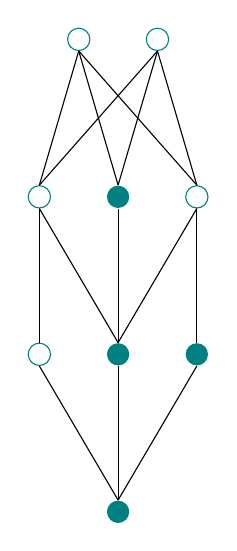
\begin{tikzpicture}[
        scale=1,
        red/.style={circle, fill=white, draw=teal, inner sep=1mm},
        blue/.style={circle, fill=teal, inner sep=1mm}]

      \node[blue] (a1) at (1.5,0){};

      \node[red] (b1) at (.5,2){};
      \node[blue] (b2) at (1.5,2){};
      \node[blue] (b3) at (2.5,2){};

      \node[red] (c1) at (.5,4){};
      \node[blue] (c2) at (1.5,4){};
      \node[red] (c3) at (2.5,4){};

      \node[red] (d1) at (1,6){};
      \node[red] (d2) at (2,6){};
      
      \foreach \b/\t in {a1/b1, a1/b2, a1/b3}
        \draw (\b.north) -- (\t.south);
      \foreach \b/\t in {b1/c1, b2/c2, b2/c3, b2/c1, b3/c3}
        \draw (\b.north) -- (\t.south);
      \foreach \b/\t in {c1/d1, c1/d2, c2/d1, c2/d2, c3/d1, c3/d2}
        \draw (\b.north) -- (\t.south);

    \end{tikzpicture}
    \end{center}
  \end{column}
  \end{columns}

\end{frame}



% =========================================================================== %
\newgeometry{margin=0mm}
\begin{frame} \frametitle{\hspace{28pt}Permutation Classes - Growth Rates} 
  \begin{center}
    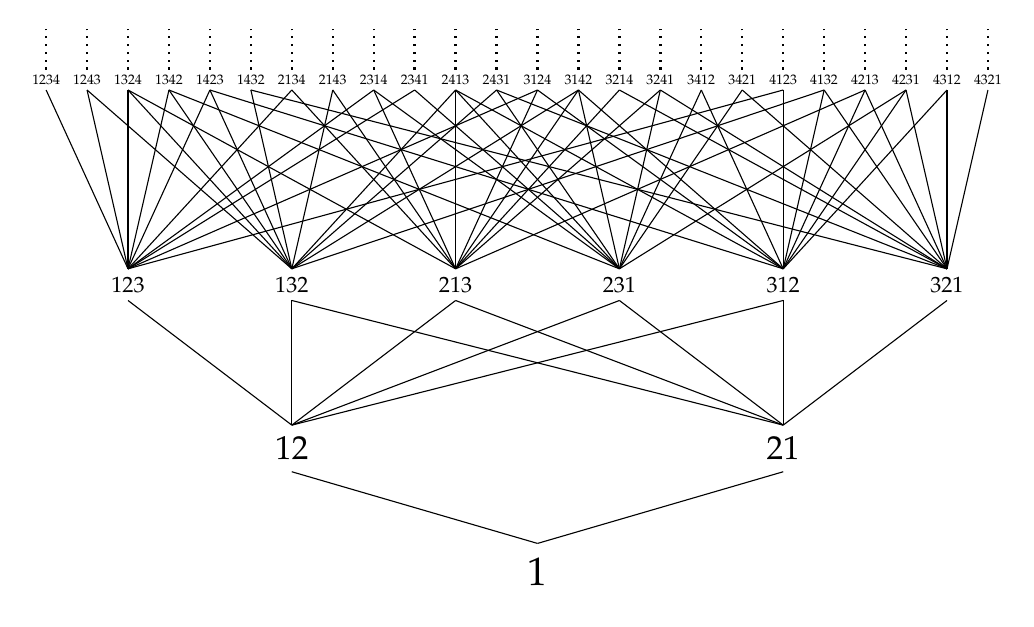
\begin{tikzpicture}[
    every node/.style={},
    scale=.52]
      {\Large
      \node (1) at (12,0) {1};
      }


      {\large
      \node (12) at (6,3) {12};
      \node (21) at (18,3) {21};
      }


      \draw (12.south)-- (1.north);
      \draw (21.south) -- (1.north);


      {\footnotesize
      \node (123) at (2 ,7) {123};
      \node (132) at (6 ,7) {132};
      \node (213) at (10,7) {213};
      \node (231) at (14,7) {231};
      \node (312) at (18,7) {312};
      \node (321) at (22,7) {321};
      }

      \draw (123.south) -- (12.north);
      \draw (132.south) -- (12.north);
      \draw (213.south) -- (12.north);
      \draw (231.south) -- (12.north);
      \draw (312.south) -- (12.north);
      
      \draw (132.south) -- (21.north);
      \draw (213.south) -- (21.north);
      \draw (231.south) -- (21.north);
      \draw (312.south) -- (21.north);
      \draw (321.south) -- (21.north);

      {\tiny
      \node (1234) at (0 ,12) {1234};
      \node (1243) at (1 ,12) {1243};
      \node (1324) at (2 ,12) {1324};
      \node (1342) at (3 ,12) {1342};
      \node (1423) at (4 ,12) {1423};
      \node (1432) at (5 ,12) {1432};

      \node (2134) at (6 ,12) {2134};
      \node (2143) at (7 ,12) {2143};
      \node (2314) at (8 ,12) {2314};
      \node (2341) at (9 ,12) {2341};
      \node (2413) at (10,12) {2413};
      \node (2431) at (11,12) {2431};

      \node (3124) at (12,12) {3124};
      \node (3142) at (13,12) {3142};
      \node (3214) at (14,12) {3214};
      \node (3241) at (15,12) {3241};
      \node (3412) at (16,12) {3412};
      \node (3421) at (17,12) {3421};

      \node (4123) at (18,12) {4123};
      \node (4132) at (19,12) {4132};
      \node (4213) at (20,12) {4213};
      \node (4231) at (21,12) {4231};
      \node (4312) at (22,12) {4312};
      \node (4321) at (23,12) {4321};
      }

      % 123
      \foreach \p in {1234, 1243, 1324, 1342, 1423, 2134, 2314, 2341, 3124, 4123}
        \draw (\p.south) -- (123.north);
      % 132
      \foreach \p in {1243, 1324, 1342, 1423, 1432, 2143, 2413, 2431, 3142, 4132}
        \draw (\p.south) -- (132.north);
      % 213
      \foreach \p in {1324, 2134, 2143, 2314, 2413, 3124, 3142, 3214, 3241, 4213}
        \draw (\p.south) -- (213.north);
      % 231
      \foreach \p in {1342, 2314, 2341, 2413, 2431, 3142, 3241, 3412, 3421, 4231}
        \draw (\p.south) -- (231.north);
      % 312
      \foreach \p in {1423, 2413, 3124, 3142, 3412, 4123, 4132, 4213, 4231, 4312}
        \draw (\p.south) -- (312.north);
      % 321
      \foreach \p in {4321, 3421, 4231, 2431, 3241, 4312, 4132, 1432, 4213, 3214}
        \draw (\p.south) -- (321.north);

      \foreach \p in {1234, 1243, 1324, 1342, 1423, 1432,
                      2134, 2143, 2314, 2341, 2413, 2431,
                      3124, 3142, 3214, 3241, 3412, 3421,
                      4123, 4132, 4213, 4231, 4312, 4321}
        \draw[dotted, line width=.3mm] (\p.north) -- ++(0,1);

    \end{tikzpicture}
  \end{center}
\end{frame}
\restoregeometry



% =========================================================================== %
\newgeometry{margin=0mm}
\begin{frame} \frametitle{\hspace{28pt}Permutation Classes - Growth Rates} 
  \begin{center}
    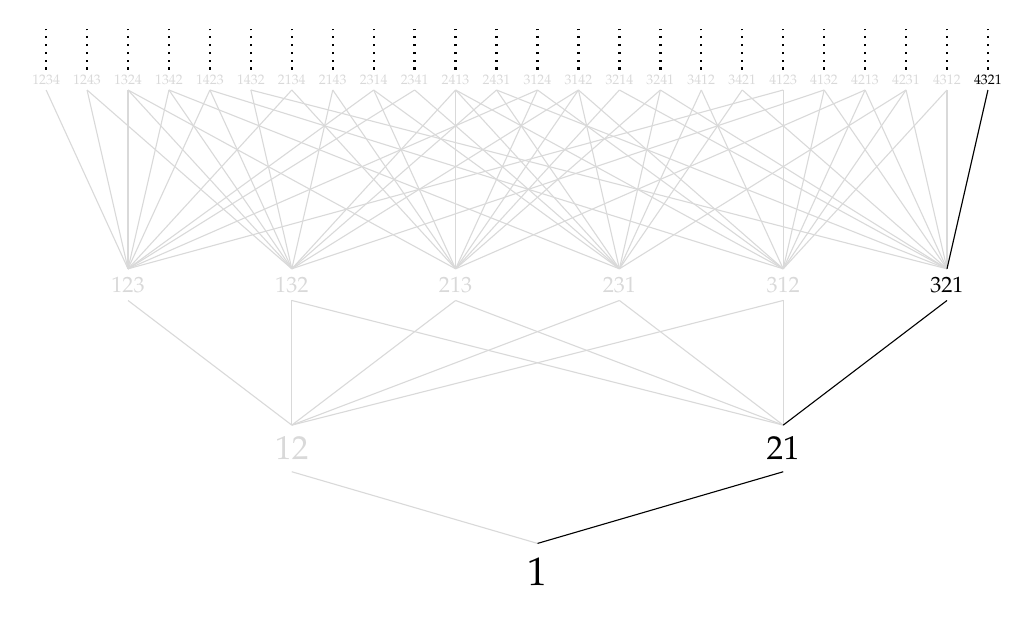
\begin{tikzpicture}[
    every node/.style={},
    scale=.52]
      {\Large
      \node (1) at (12,0) {1};
      }


      {\large
      \node (12) at (6,3) {\color{lg}{12}};
      \node (21) at (18,3) {21};
      }


      \draw[color=lg] (12.south)-- (1.north);
      \draw (21.south) -- (1.north);


      {\footnotesize
      \node (123) at (2 ,7) {\color{lg}{123}};
      \node (132) at (6 ,7) {\color{lg}{132}};
      \node (213) at (10,7) {\color{lg}{213}};
      \node (231) at (14,7) {\color{lg}{231}};
      \node (312) at (18,7) {\color{lg}{312}};
      \node (321) at (22,7) {321};
      }

      \draw[color=lg] (123.south) -- (12.north);
      \draw[color=lg] (132.south) -- (12.north);
      \draw[color=lg] (213.south) -- (12.north);
      \draw[color=lg] (231.south) -- (12.north);
      \draw[color=lg] (312.south) -- (12.north);
      
      \draw[color=lg] (132.south) -- (21.north);
      \draw[color=lg] (213.south) -- (21.north);
      \draw[color=lg] (231.south) -- (21.north);
      \draw[color=lg] (312.south) -- (21.north);
      \draw (321.south) -- (21.north);

      {\tiny
      \node (1234) at (0 ,12) {\color{lg}{1234}};
      \node (1243) at (1 ,12) {\color{lg}{1243}};
      \node (1324) at (2 ,12) {\color{lg}{1324}};
      \node (1342) at (3 ,12) {\color{lg}{1342}};
      \node (1423) at (4 ,12) {\color{lg}{1423}};
      \node (1432) at (5 ,12) {\color{lg}{1432}};

      \node (2134) at (6 ,12) {\color{lg}{2134}};
      \node (2143) at (7 ,12) {\color{lg}{2143}};
      \node (2314) at (8 ,12) {\color{lg}{2314}};
      \node (2341) at (9 ,12) {\color{lg}{2341}};
      \node (2413) at (10,12) {\color{lg}{2413}};
      \node (2431) at (11,12) {\color{lg}{2431}};

      \node (3124) at (12,12) {\color{lg}{3124}};
      \node (3142) at (13,12) {\color{lg}{3142}};
      \node (3214) at (14,12) {\color{lg}{3214}};
      \node (3241) at (15,12) {\color{lg}{3241}};
      \node (3412) at (16,12) {\color{lg}{3412}};
      \node (3421) at (17,12) {\color{lg}{3421}};

      \node (4123) at (18,12) {\color{lg}{4123}};
      \node (4132) at (19,12) {\color{lg}{4132}};
      \node (4213) at (20,12) {\color{lg}{4213}};
      \node (4231) at (21,12) {\color{lg}{4231}};
      \node (4312) at (22,12) {\color{lg}{4312}};
      \node (4321) at (23,12) {4321};
      }

      % 123
      \foreach \p in {1234, 1243, 1324, 1342, 1423, 2134, 2314, 2341, 3124, 4123}
        \draw[color=lg] (\p.south) -- (123.north);
      % 132
      \foreach \p in {1243, 1324, 1342, 1423, 1432, 2143, 2413, 2431, 3142, 4132}
        \draw[color=lg] (\p.south) -- (132.north);
      % 213
      \foreach \p in {1324, 2134, 2143, 2314, 2413, 3124, 3142, 3214, 3241, 4213}
        \draw[color=lg] (\p.south) -- (213.north);
      % 231
      \foreach \p in {1342, 2314, 2341, 2413, 2431, 3142, 3241, 3412, 3421, 4231}
        \draw[color=lg] (\p.south) -- (231.north);
      % 312
      \foreach \p in {1423, 2413, 3124, 3142, 3412, 4123, 4132, 4213, 4231, 4312}
        \draw[color=lg] (\p.south) -- (312.north);
      % 321
      \foreach \p in {4321, 3421, 4231, 2431, 3241, 4312, 4132, 1432, 4213, 3214}
        \draw[color=lg] (\p.south) -- (321.north);
      \draw (321.north) -- (4321.south);

      \foreach \p in {1234, 1243, 1324, 1342, 1423, 1432,
                      2134, 2143, 2314, 2341, 2413, 2431,
                      3124, 3142, 3214, 3241, 3412, 3421,
                      4123, 4132, 4213, 4231, 4312, 4321}
        \draw[dotted, line width=.3mm] (\p.north) -- ++(0,1);

    \end{tikzpicture}
  \end{center}
\end{frame}
\restoregeometry

% =========================================================================== %
\newgeometry{margin=0mm}
\begin{frame} \frametitle{\hspace{28pt}Permutation Classes - Growth Rates} 
  \begin{center}
    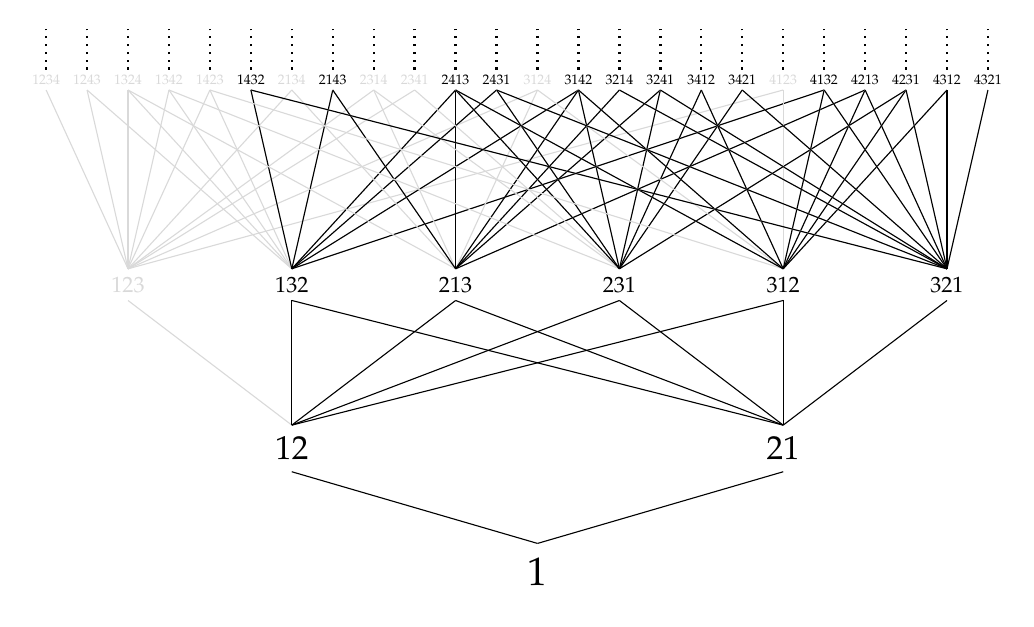
\begin{tikzpicture}[
    every node/.style={},
    scale=.52]
      {\Large
      \node (1) at (12,0) {1};
      }


      {\large
      \node (12) at (6,3) {12};
      \node (21) at (18,3) {21};
      }


      \draw (12.south)-- (1.north);
      \draw (21.south) -- (1.north);


      {\footnotesize
      \node (123) at (2 ,7) {\color{lg}{123}};
      \node (132) at (6 ,7) {132};
      \node (213) at (10,7) {213};
      \node (231) at (14,7) {231};
      \node (312) at (18,7) {312};
      \node (321) at (22,7) {321};
      }

      \draw[color=lg] (123.south) -- (12.north);
      \draw (132.south) -- (12.north);
      \draw (213.south) -- (12.north);
      \draw (231.south) -- (12.north);
      \draw (312.south) -- (12.north);
      
      \draw (132.south) -- (21.north);
      \draw (213.south) -- (21.north);
      \draw (231.south) -- (21.north);
      \draw (312.south) -- (21.north);
      \draw (321.south) -- (21.north);

      {\tiny
      \node (1234) at (0 ,12) {\color{lg}{1234}};
      \node (1243) at (1 ,12) {\color{lg}{1243}};
      \node (1324) at (2 ,12) {\color{lg}{1324}};
      \node (1342) at (3 ,12) {\color{lg}{1342}};
      \node (1423) at (4 ,12) {\color{lg}{1423}};
      \node (1432) at (5 ,12) {1432};

      \node (2134) at (6 ,12) {\color{lg}{2134}};
      \node (2143) at (7 ,12) {2143};
      \node (2314) at (8 ,12) {\color{lg}{2314}};
      \node (2341) at (9 ,12) {\color{lg}{2341}};
      \node (2413) at (10,12) {2413};
      \node (2431) at (11,12) {2431};

      \node (3124) at (12,12) {\color{lg}{3124}};
      \node (3142) at (13,12) {3142};
      \node (3214) at (14,12) {3214};
      \node (3241) at (15,12) {3241};
      \node (3412) at (16,12) {3412};
      \node (3421) at (17,12) {3421};

      \node (4123) at (18,12) {\color{lg}{4123}};
      \node (4132) at (19,12) {4132};
      \node (4213) at (20,12) {4213};
      \node (4231) at (21,12) {4231};
      \node (4312) at (22,12) {4312};
      \node (4321) at (23,12) {4321};
      }

      % 123
      \foreach \p in {1234, 1243, 1324, 1342, 1423, 2134, 2314, 2341, 3124, 4123}
        \draw[color=lg] (\p.south) -- (123.north);
      % 132
      \foreach \p in {1243, 1324, 1342, 1423, 1432, 2143, 2413, 2431, 3142, 4132}
        \draw[color=lg] (\p.south) -- (132.north);

      \foreach \p in {1432, 2143, 2413, 2431, 3142, 4132}
        \draw[] (\p.south) -- (132.north);

      % 213
      \foreach \p in {1324, 2134, 2143, 2314, 2413, 3124, 3142, 3214, 3241, 4213}
        \draw[color=lg] (\p.south) -- (213.north);

      \foreach \p in {2143, 2413, 3142, 3214, 3241, 4213}
        \draw[] (\p.south) -- (213.north);

      % 231
      \foreach \p in {1342, 2314, 2341, 2413, 2431, 3142, 3241, 3412, 3421, 4231}
        \draw[color=lg] (\p.south) -- (231.north);

      \foreach \p in {2413, 2431, 3142, 3241, 3412, 3421, 4231}
        \draw[] (\p.south) -- (231.north);

      % 312
      \foreach \p in {1423, 2413, 3124, 3142, 3412, 4123, 4132, 4213, 4231, 4312}
        \draw[color=lg] (\p.south) -- (312.north);

      \foreach \p in {2413, 3142, 3412, 4132, 4213, 4231, 4312}
        \draw[] (\p.south) -- (312.north);

      % 321
      \foreach \p in {4321, 3421, 4231, 2431, 3241, 4312, 4132, 1432, 4213, 3214}
        \draw[color=lg] (\p.south) -- (321.north);

      \foreach \p in {4321, 3421, 4231, 2431, 3241, 4312, 4132, 1432, 4213, 3214}
        \draw[] (\p.south) -- (321.north);


      \foreach \p in {1234, 1243, 1324, 1342, 1423, 1432,
                      2134, 2143, 2314, 2341, 2413, 2431,
                      3124, 3142, 3214, 3241, 3412, 3421,
                      4123, 4132, 4213, 4231, 4312, 4321}
        \draw[dotted, line width=.3mm] (\p.north) -- ++(0,1);

    \end{tikzpicture}
  \end{center}
\end{frame}
\restoregeometry



% =========================================================================== %
\newgeometry{margin=0mm}
\begin{frame} \frametitle{\hspace{28pt}Permutation Classes - Growth Rates} 
  \begin{center}
    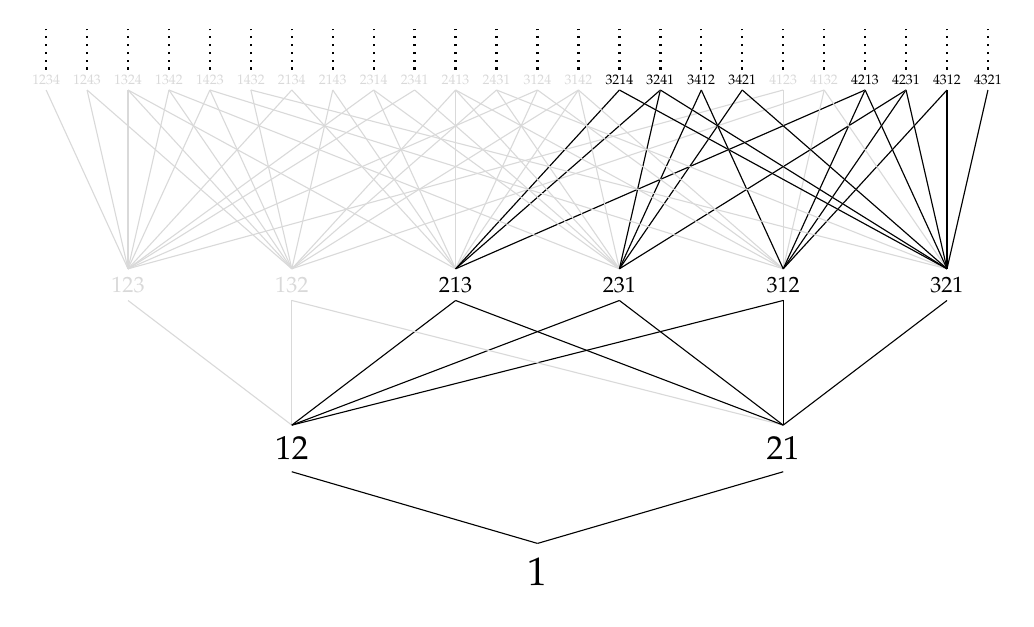
\begin{tikzpicture}[
    every node/.style={},
    scale=.52]
      {\Large
      \node (1) at (12,0) {1};
      }


      {\large
      \node (12) at (6,3) {12};
      \node (21) at (18,3) {21};
      }


      \draw (12.south)-- (1.north);
      \draw (21.south) -- (1.north);


      {\footnotesize
      \node (123) at (2 ,7) {\color{lg}{123}};
      \node (132) at (6 ,7) {\color{lg}{132}};
      \node (213) at (10,7) {213};
      \node (231) at (14,7) {231};
      \node (312) at (18,7) {312};
      \node (321) at (22,7) {321};
      }

      \draw[color=lg] (123.south) -- (12.north);
      \draw[color=lg] (132.south) -- (12.north);
      \draw (213.south) -- (12.north);
      \draw (231.south) -- (12.north);
      \draw (312.south) -- (12.north);
      
      \draw[color=lg] (132.south) -- (21.north);
      \draw (213.south) -- (21.north);
      \draw (231.south) -- (21.north);
      \draw (312.south) -- (21.north);
      \draw (321.south) -- (21.north);

      {\tiny
      \node (1234) at (0 ,12) {\color{lg}{1234}};
      \node (1243) at (1 ,12) {\color{lg}{1243}};
      \node (1324) at (2 ,12) {\color{lg}{1324}};
      \node (1342) at (3 ,12) {\color{lg}{1342}};
      \node (1423) at (4 ,12) {\color{lg}{1423}};
      \node (1432) at (5 ,12) {\color{lg}{1432}};

      \node (2134) at (6 ,12) {\color{lg}{2134}};
      \node (2143) at (7 ,12) {\color{lg}{2143}};
      \node (2314) at (8 ,12) {\color{lg}{2314}};
      \node (2341) at (9 ,12) {\color{lg}{2341}};
      \node (2413) at (10,12) {\color{lg}{2413}};
      \node (2431) at (11,12) {\color{lg}{2431}};

      \node (3124) at (12,12) {\color{lg}{3124}};
      \node (3142) at (13,12) {\color{lg}{3142}};
      \node (3214) at (14,12) {3214};
      \node (3241) at (15,12) {3241};
      \node (3412) at (16,12) {3412};
      \node (3421) at (17,12) {3421};

      \node (4123) at (18,12) {\color{lg}{4123}};
      \node (4132) at (19,12) {\color{lg}{4132}};
      \node (4213) at (20,12) {4213};
      \node (4231) at (21,12) {4231};
      \node (4312) at (22,12) {4312};
      \node (4321) at (23,12) {4321};
      }


      % 123
      \foreach \p in {1234, 1243, 1324, 1342, 1423, 2134, 2314, 2341, 3124, 4123}
        \draw[color=lg] (\p.south) -- (123.north);
      % 132
      \foreach \p in {1243, 1324, 1342, 1423, 1432, 2143, 2413, 2431, 3142, 4132}
        \draw[color=lg] (\p.south) -- (132.north);

      % 213
      \foreach \p in {1324, 2134, 2143, 2314, 2413, 3124, 3142, 3214, 3241, 4213}
        \draw[color=lg] (\p.south) -- (213.north);

      \foreach \p in {3214, 3241, 4213}
        \draw[] (\p.south) -- (213.north);

      % 231
      \foreach \p in {1342, 2314, 2341, 2413, 2431, 3142, 3241, 3412, 3421, 4231}
        \draw[color=lg] (\p.south) -- (231.north);

      \foreach \p in {3241, 3412, 3421, 4231}
        \draw[] (\p.south) -- (231.north);

      % 312
      \foreach \p in {1423, 2413, 3124, 3142, 3412, 4123, 4132, 4213, 4231, 4312}
        \draw[color=lg] (\p.south) -- (312.north);

      \foreach \p in {3412, 4213, 4231, 4312}
        \draw[] (\p.south) -- (312.north);

      % 321
      \foreach \p in {4321, 3421, 4231, 2431, 3241, 4312, 4132, 1432, 4213, 3214}
        \draw[color=lg] (\p.south) -- (321.north);

      \foreach \p in {4321, 3421, 4231, 3241, 4312, 4213, 3214}
        \draw[] (\p.south) -- (321.north);



      \foreach \p in {1234, 1243, 1324, 1342, 1423, 1432,
                      2134, 2143, 2314, 2341, 2413, 2431,
                      3124, 3142, 3214, 3241, 3412, 3421,
                      4123, 4132, 4213, 4231, 4312, 4321}
        \draw[dotted, line width=.3mm] (\p.north) -- ++(0,1);

    \end{tikzpicture}
  \end{center}
\end{frame}
\restoregeometry

\begin{frame}\frametitle{The class $\Av(132)$}

  \begin{block}{Definition}
    Let $c_n$ be the number of permutations of length $n$ which \emph{avoid}
    the pattern $132$, and $ C(x) = \sum_{n \geq 0} c_n x^n$.
  \end{block}

  \pause     

  \begin{block}{Question}
    What does a $132$-avoiding permutation look like?
  \end{block}

  \pause

  \begin{center}
  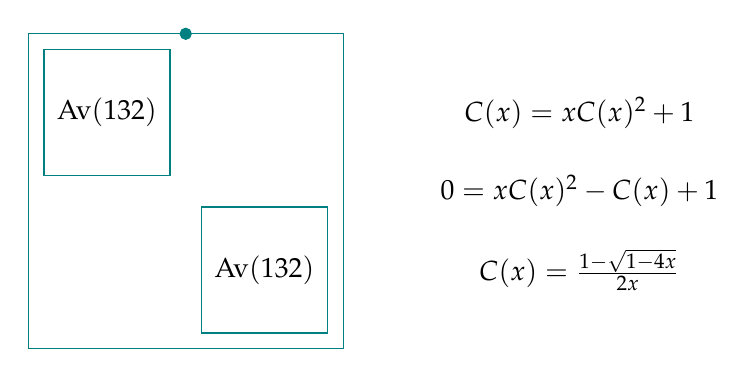
\begin{tikzpicture}[%
    scale=.2,
    filled/.style={circle, fill=teal, draw=teal, inner sep=.5mm}]

    \draw[color=teal] (0,0) -- (0,20) -- (20,20) -- (20, 0) -- cycle;
    \pause 
    \node[filled] at (10,20) {};
    \pause 

    \draw[color = teal] (1,11) -- (9,11) -- (9,19) -- (1,19) -- cycle;
    \draw[color = teal] (11, 1) -- (19,1) -- (19, 9) -- (11,9) -- cycle; 
    \pause

    \node at (5,15) {$\Av(132)$};
    \node at (15,5) {$\Av(132)$};

    \pause 
    \node at (35,15) {$C(x) = x C(x)^2 + 1$};
    \pause
    \node at (35,10) {$0 = x C(x)^2 - C(x) + 1$};
    \pause
    \node at (35, 5) {$C(x) = \frac{1 - \sqrt{1 - 4x}}{2x}$};

  \end{tikzpicture}
  \end{center}
\end{frame} 


\begin{frame} \frametitle{Lattice Paths}
  \pause

  \begin{block}{Definition}
    A \emph{NS Lattice path} of length $2n$ (or semilength $n$) is a sequence
    of vectors from the set $\{ \langle 1,1 \rangle, \langle 1, -1 \rangle \}$
    such that their sum is $\langle 2n, 0 \rangle$. 
  \end{block}

\end{frame}

\begin{frame} \frametitle{Lattice Paths}
  \pause
  \begin{center}
  \begin{tikzpicture}
    [dot/.style={circle, inner sep = 1mm,  fill = teal},
    scale = .8]
    \draw (0,0) -- (10,0);
    \pause
    \draw[->, >= latex] (0,0) -- (1,1);
    \pause
    \draw[->, >= latex] (1,1) -- (2,2);
    \pause
    \draw[->, >= latex] (2,2) -- (3,1);
    \pause
    \draw[->, >= latex] (3,1) -- (4,0);
    \pause
    \draw[->, >= latex] (4,0) -- (5,-1);
    \pause
    \draw[->, >= latex] (5,-1) -- (6,-2);
    \pause
    \draw[->, >= latex] (6,-2) -- (7,-1);
    \pause
    \draw[->, >= latex] (7,-1) -- (8,-2);
    \pause
    \draw[->, >= latex] (8,-2) -- (9,-1);
    \pause
    \draw[->, >= latex] (9,-1) -- (10,0);
  \end{tikzpicture}

  \vspace{2pc}
  \uncover<13->{
  \begin{tikzpicture}
    [dot/.style={circle, inner sep = 1mm,  fill = teal},
    scale = .8]
    \draw (0,0) -- (10,0);
    \pause
    \draw[->, >= latex] (0,0) -- (1,1);
    \pause
    \draw[->, >= latex] (1,1) -- (2,2);
    \pause
    \draw[->, >= latex] (2,2) -- (3,3);
    \pause
    \draw[->, >= latex] (3,3) -- (4,2);
    \pause
    \draw[->, >= latex] (4,2) -- (5,1);
    \pause
    \draw[->, >= latex] (5,1) -- (6,2);
    \pause
    \draw[->, >= latex] (6,2) -- (7,1);
    \pause
    \draw[->, >= latex] (7,1) -- (8,2);
    \pause
    \draw[->, >= latex] (8,2) -- (9,1);
    \pause
    \draw[->, >= latex] (9,1) -- (10,0);
  \end{tikzpicture}
  }

  \end{center}
\end{frame}

\begin{frame} \frametitle{Lattice Paths}
  \begin{block}{Questions}    
  \pause
  \begin{itemize}
    \item[Q1)] How many NS lattice paths are there of semilength $n$?
    \pause
    \item[A1)] $\displaystyle \binom{2n}{n}$. 
    \pause
    \item[Q2)] How many NS lattice paths are there of semilength $n$ which
    never pass below the line $y=0$? 
  \end{itemize}
  \end{block}

\end{frame}

\begin{frame} \frametitle{Dyck Paths}
  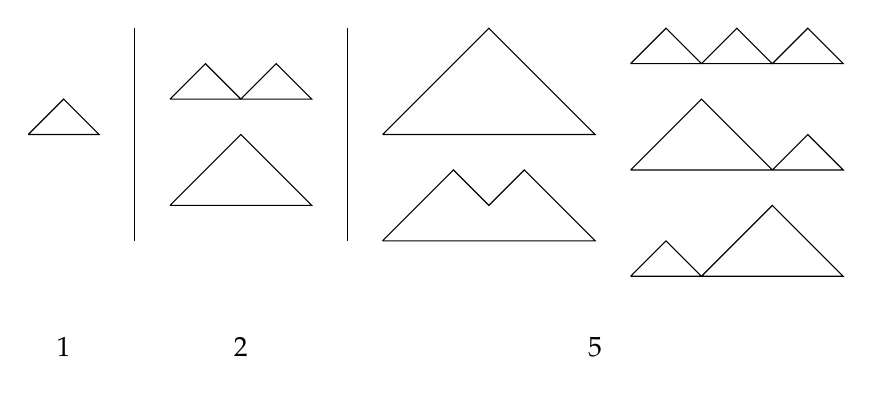
\begin{tikzpicture}
    [dot/.style={circle, inner sep = 1mm,  fill = teal},
    scale = .45]

    \node at (1, -6) {1};
    \draw (0,0) -- (2,0) -- (1,1) -- (0,0);

    \pause
    \draw (3,3) -- (3,-3);
    \node at (6, -6) {2};
    \draw (4, 1) -- (8,1) -- (7, 2) -- (6,1) -- (5,2) -- (4,1);
    \draw (4, -2) -- (8,-2) -- (7, -1) -- (6,0) -- (5,-1) -- (4,-2);

    \pause
    \draw (9,3) -- (9,-3);
    \node at (16, -6) {5};
    \draw (10, 0) -- (16, 0) -- (13,3) -- (10,0);
    \draw (10, -3) -- (16, -3) -- (14,-1) -- (13, -2) -- (12, -1) --(10, -3);
    \draw (17, 2) -- (23 , 2) -- (22,3)--(21,2)--(20,3)--(19,2)--(18,3)--(17,2);
    \draw (17,-1)--(19,1)--(21,-1)--(22,0)--(23,-1)--(17,-1);
    \draw (17,-4)--(18,-3)--(19,-4)--(21,-2)--(23,-4)--(17,-4);

  \end{tikzpicture}
\end{frame}

\begin{frame} \frametitle{Dyck Paths}

  Let $p_n$ be the number of NS paths of length $2n$ that \emph{don't} cross
  below the $x$-axis, and let $ \ds P = \sum_{n \geq 0} p_n x^n$.
  \pause

  \vspace{1pc}

  \begin{tikzpicture}
  [scale = .6]
    \draw[color=white] (7,3)--(7,-5);
    \draw (0,0) -- (16,0);
    \draw[->, >= latex] (0,0) -- (1,1);
    
    \only<3-4>{
      \draw[->, >= latex] (1,1) -- (2,2);
      \draw[->, >= latex] (2,2) -- (3,1);
      \draw[->, >= latex] (3,1) -- (4,2);
      \draw[->, >= latex] (4,2) -- (5,3);
      \draw[->, >= latex] (5,3) -- (6,2);
      \draw[->, >= latex] (6,2) -- (7,1);
    }

    \only<5->{
      \node at (4, 2) {$P$};
      \node at (12, 1) {$P$};
      \draw (1,1) -- (7,1);
    }
    \only<4->{
      \draw (8,3) -- (8,-1);
    }

    \draw[->, >= latex] (7,1) -- (8,0);

    \only<3-4>{
      \draw[->, >= latex] (8,0) -- (9,1);
      \draw[->, >= latex] (9,1) -- (10,0);
      \draw[->, >= latex] (10,0) -- (11,1);
      \draw[->, >= latex] (11,1) -- (12,2);
      \draw[->, >= latex] (12,2) -- (13,1);
      \draw[->, >= latex] (13,1) -- (14,2);
      \draw[->, >= latex] (14,2) -- (15,1);
      \draw[->, >= latex] (15,1) -- (16,0);
    }
    \only<6->{
      \node at (3, -2) {$P = x P^2 + 1$};
    }
    \only<7->{
      \node at (9, -2) {$0 = xP^2 - P + 1$};
    }
    \only<8->{
      \node at (15, -2) {$ P = \frac{1 \pm \sqrt{1 - 4x}}{2x}$};
    }
    \only<9->{
      \node at (9, -4) {$\ds P = \frac{1 - \sqrt{1-4x}}{2x} = 
        1 + x + 2x^2 + 5x^3 + 14x^4 + \ldots $};
    }
  \end{tikzpicture}
\end{frame}

\begin{frame} \frametitle{Dyck Paths}

  Let $p_n$ be the number of NS paths of length $2n$ that \emph{don't} cross
  below the $x$-axis, and let $ \ds P = \sum_{n \geq 0} p_n x^n$.

  \vspace{1pc}

  \begin{tikzpicture}
  [scale = .6]
    \draw[color=white] (7,3)--(7,-5);
    \draw (0,0) -- (16,0);
    
    \only<1-2>{
      \draw[->, >= latex] (0,0) -- (1,1);
      \draw[->, >= latex] (1,1) -- (2,2);
      \draw[->, >= latex] (2,2) -- (3,1);
      \draw[->, >= latex] (3,1) -- (4,2);
      \draw[->, >= latex] (4,2) -- (5,3);
      \draw[->, >= latex] (5,3) -- (6,2);
      \draw[->, >= latex] (6,2) -- (7,1);
      \draw[->, >= latex] (7,1) -- (8,0);
      \draw[->, >= latex] (8,0) -- (9,1);
      \draw[->, >= latex] (9,1) -- (10,0);
      \draw[->, >= latex] (10,0) -- (11,1);
      \draw[->, >= latex] (11,1) -- (12,2);
      \draw[->, >= latex] (12,2) -- (13,1);
      \draw[->, >= latex] (13,1) -- (14,2);
      \draw[->, >= latex] (14,2) -- (15,1);
      \draw[->, >= latex] (15,1) -- (16,0);
    }

    \only<2-4>{
      \draw (8,3) -- (8,-1);
      \draw (10,3) -- (10,-1);
    }

    \only<3-4>{
      \draw[->, >= latex] (0,0) -- (1,1);
      \draw[->, >= latex] (7,1) -- (8,0);
      \draw[->, >= latex] (8,0) -- (9,1);
      \draw[->, >= latex] (9,1) -- (10,0);
      \draw[->, >= latex] (10,0) -- (11,1);
      \draw[->, >= latex] (15,1) -- (16,0);
      \node at (4,1.5) {$P$};
      \node at (9,1.5) {$P$};
      \node at (13,1.5) {$P$};
    }

    \only<5->{
      \draw[->, >= latex] (0,0) -- (1,1);
      \draw[->, >= latex] (3,1) -- (4,0);
      \draw[->, >= latex] (4,0) -- (5,1);
      \draw[->, >= latex] (7,1) -- (8,0);
      \draw[->, >= latex] (8,0) -- (9,1);
      \draw[->, >= latex] (11,1) -- (12,0);
      \draw[->, >= latex] (12,0) -- (13,1);
      \draw (4,3) -- (4,-1);
      \draw (8,3) -- (8,-1);
      \draw (12,3) -- (12,-1);
      \node at (2,1) {$P$};
      \node at (6,1) {$P$};
      \node at (10,1) {$P$};
      \node at (14,1) {$\cdots$};
    }

    \only<4>{
      \node at (8, -2) {$P = x^3 P^3$};
    }
    \only<5>{
      \node at (8, -2) {$P =  1+ xP + x^2P^2 + x^3 P^3 +x^4 P^4
      + x^5P^5 + \cdots$};
    }
    \only<6->{
      \node at (8, -2) {$P =  1 + xP + x^2P^2 + x^3P^3 + x^4P^4
      + x^5P^5 + \cdots = \displaystyle \frac{1}{1-xP}$};
    }
    \only<7->{
      \node at (3, -4) {$P(1-xP) = 1$};
    }
    \only<8->{
      \node at (9, -4) {$P = xP^2 + 1$};
    }
  \end{tikzpicture}
\end{frame}

\begin{frame} \frametitle{Catalan Numbers}
  \pause
  \begin{block}{Fact}
    $$ 
    C(x) = \frac{1 - \sqrt{1 - 4x}}{2x} 
      = \sum_{n \geq 0} \frac{1}{n+1} \binom{2n}{n} x^n.
    $$
    \pause
    The numbers $c_n = \frac{1}{n+1} \binom{2n}{n}$ are called the Catalan
    numbers. 
    The first few numbers in the sequence are
    $$ 1, 1, 2, 5, 14, 42, 132, 429, 1430, 4862 \cdots $$
  \end{block}
    
\end{frame}

\begin{frame} \frametitle{Two Catalan Recurrences}
  \pause
  $$ C(x) = xC(x)^2 + 1 \text{ \qquad and \qquad } C(x) = 1 + x C(x) + x^2 C(x) +
  \cdots$$

  \pause 
  \vspace{1pc}

  $$ c_0 = 1, \quad c_i = 0 \text{\ for $i < 0$}$$ 

  \vspace{6pt}

  $$ c_n = \sum_{i+j = n-1} c_i c_j $$

  \vspace{6pt}


  $$ c_n = c_{n-1} + \sum_{i+j = n-2} c_i c_j + \sum_{i + j + k = n-3} c_i c_j c_k
    + \cdots $$
\end{frame}

\begin{frame} \frametitle{The Class Av(123)}
  \only<1>{
  \begin{block}{Question}
    What does a $123$-avoiding permutation look like? 
  \end{block}
  }

  \begin{center}
  \uncover<2->{
    $\pi = 4\ 7\ 6\ 2\ 5\ 1\ 3$
  }

  \vspace{3pc}

  \only<3>{
  \begin{tikzpicture}
  [scale=.6, auto=center, every node/.style={circle,
  fill=black, inner sep=2pt, minimum size=2pt}]
    \foreach \x/\y in {1/4,2/7,3/6,4/2,5/5,6/1,7/3}{
      \node (p-\x) at (\x,\y) {}; }
  \end{tikzpicture} 
  }

  \only<4>{
  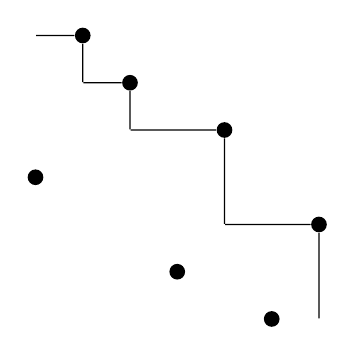
\begin{tikzpicture}
  [scale=.6, auto=center]
    \foreach \x/\y in {1/4,4/2,6/1}{
      \node[circle,fill=black,inner sep=2pt, minimum size=2pt]
      (r\x) at (\x,\y) {}; }
    \foreach \num/\x/\y in {1/2/7,2/3/6,3/5/5,4/7/3}{
      \node[circle,fill=black,inner sep=2pt, minimum size=2pt]
      (b\num) at (\x,\y) {};}
    \foreach \num/\x/\y in {1/1/7,2/2/6,3/3/5,4/5/3,5/7/1}{
      \node[circle,fill=black, inner sep=0pt, minimum size=0pt]
      (g\num) at (\x,\y) {};}
    \foreach \to/\from in {g1/b1,b1/g2,g2/b2,b2/g3,
                  g3/b3,b3/g4,g4/b4,b4/g5}{
      \draw (\to) -- (\from);}
  \end{tikzpicture} 
  }


  \only<5>{
  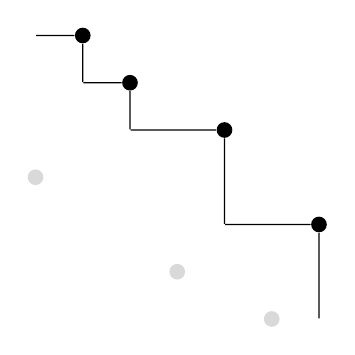
\begin{tikzpicture}
  [scale=.6, auto=center]
    \foreach \x/\y in {1/4,4/2,6/1}{
      \node[circle,fill=lg,inner sep=2pt, minimum size=2pt]
      (r\x) at (\x,\y) {}; }
    \foreach \num/\x/\y in {1/2/7,2/3/6,3/5/5,4/7/3}{
      \node[circle,fill=black,inner sep=2pt, minimum size=2pt]
      (b\num) at (\x,\y) {};}
    \foreach \num/\x/\y in {1/1/7,2/2/6,3/3/5,4/5/3,5/7/1}{
      \node[circle,fill=black, inner sep=0pt, minimum size=0pt]
      (g\num) at (\x,\y) {};}
    \foreach \to/\from in {g1/b1,b1/g2,g2/b2,b2/g3,
                  g3/b3,b3/g4,g4/b4,b4/g5}{
      \draw (\to) -- (\from);}
  \end{tikzpicture} 
  }

  \uncover<6>{
  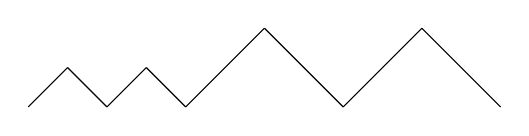
\begin{tikzpicture}
  [scale=.5, auto=center]
    \draw (0,0) -- (1,1);
    \draw (1,1) -- (2,0);
    \draw (2,0) -- (3,1);
    \draw (3,1) -- (4,0);
    \draw (4,0) -- (6,2);
    \draw (6,2) -- (8,0);
    \draw (8,0) -- (10,2);
    \draw (10,2) -- (12,0);
  \end{tikzpicture} 
  }
  \end{center}
\end{frame}


\begin{frame} 
  \begin{center}
    \rmfamily \LARGE \color{teal}{Counting Patterns}
  \end{center}
\end{frame}
    

\begin{frame}{Introduction}
  \pause 

  \begin{block}{Example}
    The permutation $3 \ 5 \ 1 \ 2 \ 4$ contains the
    pattern $3 \ 1 \ 2$ three times.
  \end{block}
  \pause

  \begin{block}{Example}
    The set $\{ 2341 , 1234, 4321 \} $ contains the pattern $123$
    exactly $5$ times. 
  \end{block}

  \pause

  \begin{block}{Notation}
    Let $\num_\si (S)$ denote the number of occurrences of $\si$ within the
    set $S$. 
  \end{block}
\end{frame}

\begin{frame} \frametitle{An Example}

  \begin{block}{Question}
    How many times does the pattern $1324$ occur within the set of all
    $n$-permutations? That is, what is 
    $$\num_{1324} (\S_n)?$$
  \end{block}
\end{frame}

\begin{frame} \frametitle{An Example}

  \begin{block}{Answer}
  Let $X$ be a random variable denoting the number of $1324$ patterns in a
  random $n$-permutation. Then $\Ex{X} = \num_{1324}(\S_n) / n!$. 
  
  \pause
  
  Let $X_{i,j,k,l}$ be the random variable equal to 0 or 1, which indicates
  whether the $i$th, $j$th, $k$th, and $l$th entries form a $1324$ pattern.
  Then 
  $$ X = \sum_{1 \leq i < j < k < l \leq n} X_{i,j,k,l} $$
  \pause
  $$ \begin{aligned}
    \Ex{X} &= \sum_{1 \leq i < j < k < l \leq n} \Ex{X_{i,j,k,l}} \pause \\
       &= \sum_{1 \leq i < j < k < l \leq n} \frac{1}{4!} \pause 
       = \binom{n}{4} \frac{1}{4!}.
    \end{aligned} $$

  Therefore 
  $$\num_{1324}(\S_n) = \binom{n}{4} \frac{n!}{4!}.$$

  \end{block}

\end{frame}


\begin{frame}{Motivation}
  \begin{block}{Fact}
    In $\S_n$, the number of occurrences of a specific pattern depends only on
    the length of the pattern. 
  \end{block}
  \pause
  \begin{block}{Question}
  How does this change when we replace $\S_n$ with a 
  proper permutation class?
  \end{block}
  \pause

  \begin{figure}
  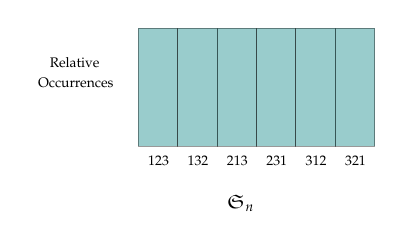
\begin{tikzpicture}
  [scale = .5]
  \foreach \x in {0,1,2,3,4,5}{
    \draw[color = black, fill = teal, opacity = .4] (\x,0) rectangle (\x+1, 3);
  }
  \draw (0, 0) node[anchor=north west] {\tiny $123$};
  \draw (1, 0) node[anchor=north west] {\tiny $132$};
  \draw (2, 0) node[anchor=north west] {\tiny $213$};
  \draw (3, 0) node[anchor=north west] {\tiny $231$};
  \draw (4, 0) node[anchor=north west] {\tiny $312$};
  \draw (5, 0) node[anchor=north west] {\tiny $321$};
  \draw (2,-1) node[anchor=north west] {\scriptsize $\S_n$};
  \draw (-2.5, 2.5) node[anchor=north west] {\tiny Relative};
  \draw (-2.8, 2) node[anchor=north west] {\tiny Occurrences};
  \end{tikzpicture} \hspace{2pc} \pause
  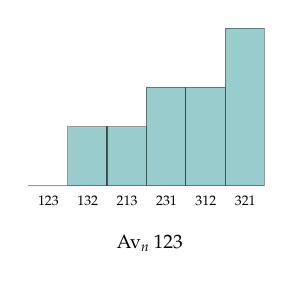
\begin{tikzpicture}
  [scale = .5]
  \foreach \x/\y in {0/0, 1/1.5, 2/1.5, 3/2.5, 4/2.5, 5/4}{
    \draw[color = black, fill = teal, opacity = .4] (\x,0) rectangle (\x+1,\y );
  }
  \draw (0, 0) node[anchor=north west] {\tiny $123$};
  \draw (1, 0) node[anchor=north west] {\tiny $132$};
  \draw (2, 0) node[anchor=north west] {\tiny $213$};
  \draw (3, 0) node[anchor=north west] {\tiny $231$};
  \draw (4, 0) node[anchor=north west] {\tiny $312$};
  \draw (5, 0) node[anchor=north west] {\tiny $321$};
  \draw (2,-1) node[anchor=north west] {\scriptsize $\Av_n 123$};
  \end{tikzpicture}
  \end{figure}
\end{frame}


  %\begin{frame}{Notation}
  %  \pause
  %
  %  \begin{block}{Definition}
  %    For any permutations $q$ and $p$, denote by $\num_q (p)$ the
  %    number of occurrences of the pattern $q$ in the permutation $p$. 
  %  \end{block}
  %  \pause
  %  
  %  \begin{block}{Example}
  %    $$ \num_{21} (23154) = 3$$
  %  \end{block}
  %
  %  \pause
  %  
  %  \begin{block}{Definition}
  %    Similarly, for a pattern $q$ and a set $S$ of permutations,
  %    define 
  %    $$ \num_q (S) = \sum_{p \in S} \num_q(p). $$
  %    \pause
  %    $$\num_{231}^{-1}(0) \cap \S_n = \frac{1}{n+1} \binom{2n}{n} = c_n$$
  %  \end{block}
  %
  %\end{frame}


\begin{frame}{Data}
  \pause
  \vspace{-1pc}
  $$ \Av 132 $$
  $$\begin{array}{c|c|c|c|c|c|c}
      \text{length} & 123 & 132 & 213 & 231
      & 312 & 321 \\
      \hline
     3  & 1     &    0  &    1 &    1 &    1 &    1  \\
     \pause
     4  & 10    &    0  &   11 &   11 &   11 &   13  \\
     \pause
     5  & 68    &    0  &   81 &   81 &   81 &  109  \\
     6  & 392   &    0  &  500 &  500 &  500 &  748  \\ 
     7  & 2063  &    0  & 2794 & 2794 & 2794 & 4570   
   \end{array}
  $$
\end{frame}

\begin{frame}{Previous Results}

  \begin{block}{Theorem (B\'ona)}
    In $\Av_n 132$, the pattern $123$ is the least common, $321$ is the most
    common, and $\num_{213} = \num_{231} = \num_{312}$. \\
  \end{block}
    
\end{frame}


\begin{frame}{Data}
  \pause
  \vspace{-1pc}
  $$ \Av 132 $$
  $$\begin{array}{c|c|c|c|c|c|c}
      \text{length} & 123 & 132 & 213 & 231
      & 312 & 321 \\
      \hline
     3  & 1     &    0  &    1 &    1 &    1 &    1  \\
     4  & 10    &    0  &   11 &   11 &   11 &   13  \\
     5  & 68    &    0  &   81 &   81 &   81 &  109  \\
     6  & 392   &    0  &  500 &  500 &  500 &  748  \\ 
     7  & 2063  &    0  & 2794 & 2794 & 2794 & 4570   
   \end{array}
  $$
  \pause
  $$\Av 123 $$
  $$\begin{array}{c|c|c|c|c|c|c}
      \text{length} & 123 & 132 & 213 & 231
      & 312 & 321 \\
      \hline
      3  & 0     &    1  &    1 &    1 &    1 &    1  \\
      \pause
      4  & 0     &    9  &    9 &   11 &   11 &   16  \\
      \pause
      5  & 0     &    57 &   57 &   81 &   81 &  144  \\
      6  & 0     &   312 &  312 &  500 &  500 & 1016  \\ 
      7  & 0     &  1578 & 1578 & 2794 & 2794 & 6271   
    \end{array}
  $$
\end{frame}

\begin{frame} 
  \begin{center}
    \rmfamily \LARGE \color{teal}{Patterns Within $\Av 123$ }
  \end{center}
\end{frame}


\begin{frame}{Patterns of Length 2}
  \pause
  \begin{block}{Theorem (Cheng, Eu, Fu)}
    $$ \num_{12}(\Av_n 123) =  4^{n-1} - \binom{2n-1}{n}.$$
    % It follows that 
    % $$\sum_{n \geq 0} \num_{12}(\Av_n 123) x^n = 
    %   \frac{1 - 2x - \sqrt{1-4x}}{2(1-4x)}.$$
    
  \end{block}

  \pause

  \begin{block}{Fact}
    $$ (\num_{12} + \num_{21})(\Avn)  = \binom{n}{2} c_n .$$ 
  \end{block}
\end{frame}

\begin{frame}{Patterns of Length 3} \pause
  
  \begin{block}{Fact}
    $$ 2 \num_{132} + 2 \num_{231} + \num_{321} = \binom{n}{3} c_n.$$
  \end{block}

  \pause

  \begin{proof}
    Rewrite the left hand side as 
    $$ \num_{132} +\num_{213} + \num_{231} + \num_{312} + \num_{321} $$
  \end{proof}

\end{frame}

\begin{frame}{Patterns of Length 3} 

  \begin{block}{Proposition}
    $$ (4 \num_{132} + 2 \num_{231})(\Avn) =
      (n-2) \num_{12}(\Avn). $$
  \end{block}
  \pause

  \begin{proof}
    Rewrite as 
    $$ (n-2)\num_{12} - \num_{132} - \num_{213} = 
      \num_{231} + \num_{312}+ \num_{132} + \num_{213}. $$
    Both sides count the number of length three patterns with at least
    one non-inversion.
  \end{proof}

\end{frame}


% \begin{frame}{Preliminaries}
% 
%   \begin{block}{Lemma}
%     Let $a_n = \num_{132}(\Avn)$, $b_n = \num_{231}(\Avn)$, $d_n =
%     \num_{321}(\Avn)$, and $j_n = \num_{12}(\Avn)$. Let $A(x), B(x),
%     D(x), J(x)$ be their respective generating functions. Then 
%     $$ \begin{array}{ccccc}
%       2A(x) & + 2B(x) & + D(x) & = & \frac{x^3}{6} (C(x))''' \\
%       4A(x) & + 2B(x) & & =&  x^3(J(x)/x^2)' 
%       \end{array} $$
%   \end{block}
% 
% \end{frame}
  

% \newgeometry{margin=0mm}
\begin{frame}{Indecomposable Permutations}
\pause
  
  \begin{block}{Definition}
    We say that a permutation $p = p_1 p_2 \ldots p_n$ is
    \emph{decomposable} if there exists an integer $k$ so that each
    of the entries $p_1, \ldots p_k$ is greater than each of the
    entries $p_{k+1}, \ldots p_n$. Otherwise, we say that $p$ is
    \emph{indecomposable}
  \end{block}

  \pause

  \begin{block}{Example}
    The permutation $3 5 6 4 1 2$ is decomposable, as the entries
    $3564$ are larger than the entries $12$
  \end{block}

  \pause

  \begin{block}{Definition}
    Denote by $\Avns$ the set of indecomposable $n$-permutations which
    avoid $123$.
  \end{block}

\end{frame}


\begin{frame}{Indecomposable Permutations}

  \begin{block}{Fact}
    $|\Avns| = c_{n-1}$.
  \end{block}
  \pause

  \begin{proof}
    \vspace{.5pc}

    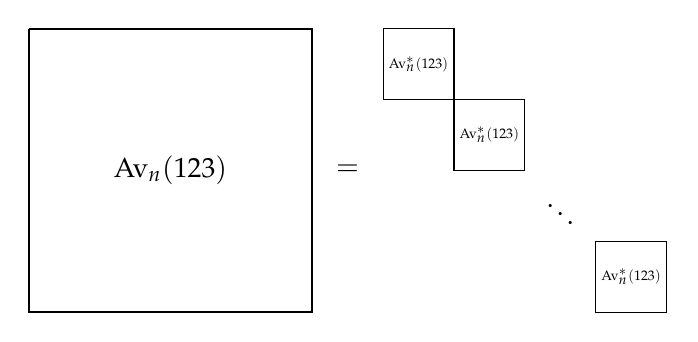
\begin{tikzpicture}[scale = .45]
      
      \draw[thick] (0,8) -- (0,0) -- (8,0) -- (8,8) -- (0,8);
      \node at (4,4) {$\Avn$};
      \node at (9,4) {$ = $};

      \draw (10,8) -- (10,6) -- (12,6) -- (12,8) -- (10,8);
      \node at (11,7) {\tiny $ \Avns$};

      \draw (12,6) -- (12,4) -- (14,4) -- (14,6) -- (12,6);
      \node at (13,5) {\tiny $ \Avns$};
      
      \node at (15,3) {$\ddots$};

      \draw (16,2) -- (16,0) -- (18,0) -- (18,2) -- (16,2);
      \node at (17,1) {\tiny $ \Avns$};
    \end{tikzpicture}

    \pause
    $$ C(x) = 1 + C^*(x) + C^*(x)^2 + \ldots = \frac{1}{1 - C^*(x)}$$

    \vspace{-.5pc}
    \pause
    $$ C^*(x) = \frac{C(x) - 1}{C(x)} = \frac{(xC(x)^2 + 1) - 1}{C(x)}=  xC(x).$$


  \end{proof}

\end{frame}


\begin{frame}{Indecomposable Permutations}

  \begin{block}{Fact}
    $|\Avns| = c_{n-1}$.
  \end{block}

  \begin{proof}[Alternate Proof]
    \vspace{.5pc}

    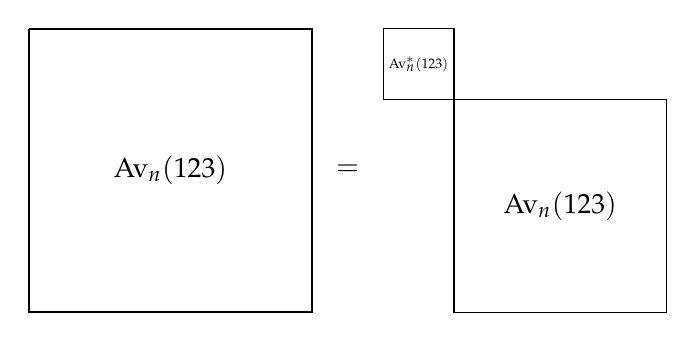
\begin{tikzpicture}[scale = .45]
      
      \draw[thick] (0,8) -- (0,0) -- (8,0) -- (8,8) -- (0,8);
      \node at (4,4) {$\Avn$};
      \node at (9,4) {$ = $};

      \draw (10,8) -- (10,6) -- (12,6) -- (12,8) -- (10,8);
      \node at (11,7) {\tiny $ \Avns$};

      \draw (12,6) -- (12,0) -- (18,0) -- (18,6) -- (12,6);
      \node at (15,3) {$ \Avn$};
    \end{tikzpicture}

    $$ C(x) = C^*(x) C(x) + 1$$
    
    \vspace{-.5pc}
    $$ C^*(x) = \frac{C(x) - 1}{C(x)} = \frac{(xC(x)^2 + 1) - 1}{C(x)}=  xC(x).$$


  \end{proof}

\end{frame}
% \restoregeometry


% \begin{frame}
%   \begin{block}{Lemma}
%     Let $a_n = \num_{132}(\Avn)$, $b_n = \num_{231}(\Avn)$, $d_n =
%     \num_{321}(\Avn)$, and $j_n = \num_{12}(\Avn)$. Let $A(x), B(x),
%     D(x), J(x)$ be their respective generating functions. Let $*$
%     denote the corresponding numbers for indecomposable permutations.
%     Then 
%     $$ \begin{array}{ccccc}
%       2A(x) & + 2B(x) & + D(x) & = & \frac{x^3}{6} (C(x))''' \\
%       4A(x) & + 2B(x) & & =&  x^3(J(x)/x^2)' \\
%       \pause
%       2A^*(x) & + 2B^*(x) & + D^*(x) & = & \frac{x^3}{6} (xC(x))'''\\
%       4A^*(x)& + 2B^*(x)& & =& x^3(J^*(x) /x^2)' 
%       \end{array} $$
%   \end{block}
% 
% \end{frame}


\begin{frame}{Solving the System}
  \begin{block}{\only<-2>{Conjectures}\uncover<3>{Corollary}}
    \pause
    $$ C(x) A(x)  = xJ(x) C'(x)$$
    % $$ C(x) A^*(x) = xF^*(x) C'(x) $$
    $$ A^*(x) + B^*(x) = \sum_{n\geq 0} \num_{213} \big(\Av_n^* 132
    \big) x^n $$ 
    $$ B^*(x) C(x) = 2xB(x) $$
    $$ A(x)+B(x) = 2\sum_{n\geq 0} \Big(\num_{213} \big( \Av ^*_n
    132 \big) + \num_{231} \big( \Av ^*_n 132 \big)\Big) x^n $$
    $$ A(x) + B(x) = xB^*(x) $$
    $$ J^*(x)  = 2A^*(x) $$
  \end{block}
\end{frame}


\begin{frame} \frametitle{The Lemma}
\pause

  \begin{block}{Lemma}
    $$A^*(x) = \frac{x^3C(x)}{(1-4x)^{3/2}}$$
  \end{block}

\end{frame}





\begin{frame}{Sketch of proof}

  \only<-12>{
    Let $p = 4 \ 3 \ 7 \ 6 \ 1 \ 5 \ 2 $, and count $213$ patterns. \\
    \hfill 
  }
  \only<13->{ Let $h_{n,k}$ denote the total number of peaks at height
  $k$ in all Dyck paths of semilength $n$. 
  Let $H(x,u) = \sum_{n,k \geq 0} h_{n,k} x^n u^k$. \\
  \vspace{-.4pc} }

  \begin{figure}[center]
  
  % lots of pictures... not the prettiest code
    \only<1>{
      \begin{tikzpicture}[scale = .7, auto = center]
        \draw[thick, color =  white] (0,8) -- (0,0) -- (8,0);
      \end{tikzpicture}
      }

    \only<2>{
      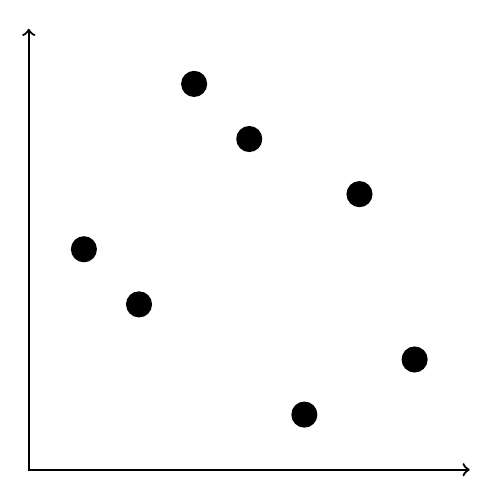
\begin{tikzpicture}[scale = .7, auto = center]
        \draw[thick, <->] (0,8) -- (0,0) -- (8,0);
        \node[circle, fill=black] at (1,4) {};
        \node[circle, fill=black] at (2,3) {};
        \node[circle, fill=black] at (3,7) {};
        \node[circle, fill=black] at (4,6) {};
        \node[circle, fill=black] at (5,1) {};
        \node[circle, fill=black] at (6,5) {};
        \node[circle, fill=black] at (7,2) {};
      \end{tikzpicture}
    }

    \only<3>{ 
      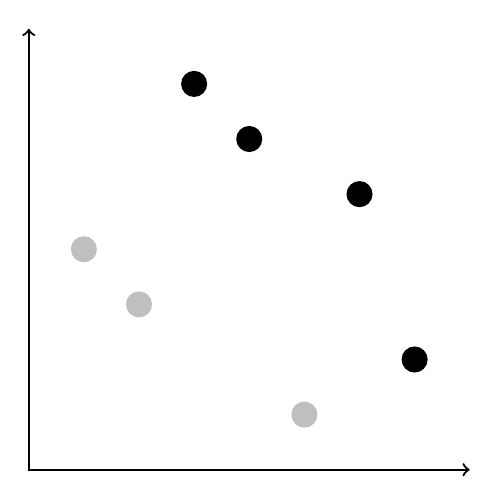
\begin{tikzpicture}[scale = .7, auto = center]
        \draw[thick, <->] (0,8) -- (0,0) -- (8,0);
        \node[circle, fill=lightgray] at (1,4) {};
        \node[circle, fill=lightgray] at (2,3) {};
        \node[circle, fill=black] at (3,7) {};
        \node[circle, fill=black] at (4,6) {};
        \node[circle, fill=lightgray] at (5,1) {};
        \node[circle, fill=black] at (6,5) {};
        \node[circle, fill=black] at (7,2) {};
      \end{tikzpicture}
    }

    \only<4>{ 
      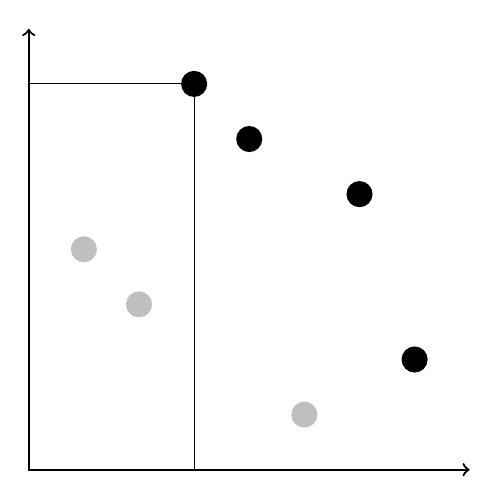
\begin{tikzpicture}[scale = .7, auto = center]
        \draw[thick, <->] (0,8) -- (0,0) -- (8,0);
        \node[circle, fill=lightgray] at (1,4) {};
        \node[circle, fill=lightgray] at (2,3) {};
        \node[circle, fill=black] at (3,7) {};
        \node[circle, fill=black] at (4,6) {};
        \node[circle, fill=lightgray] at (5,1) {};
        \node[circle, fill=black] at (6,5) {};
        \node[circle, fill=black] at (7,2) {};
        \draw (0,7) -- (3,7) -- (3,0);
      \end{tikzpicture}
    }

    \only<5>{ 
      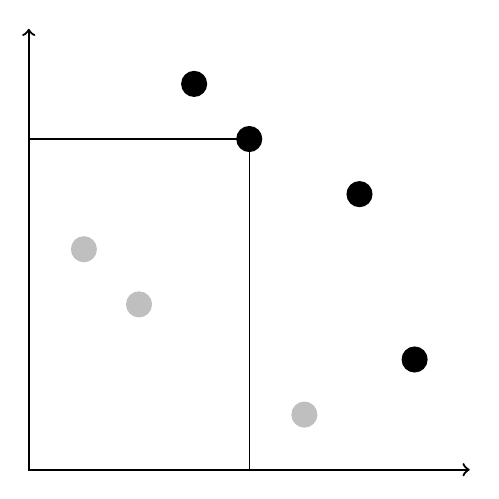
\begin{tikzpicture}[scale = .7, auto = center]
        \draw[thick, <->] (0,8) -- (0,0) -- (8,0);
        \node[circle, fill=lightgray] at (1,4) {};
        \node[circle, fill=lightgray] at (2,3) {};
        \node[circle, fill=black] at (3,7) {};
        \node[circle, fill=black] at (4,6) {};
        \node[circle, fill=lightgray] at (5,1) {};
        \node[circle, fill=black] at (6,5) {};
        \node[circle, fill=black] at (7,2) {};
        \draw (0,6) -- (4,6) -- (4,0);
      \end{tikzpicture}
    }

    \only<6>{ 
      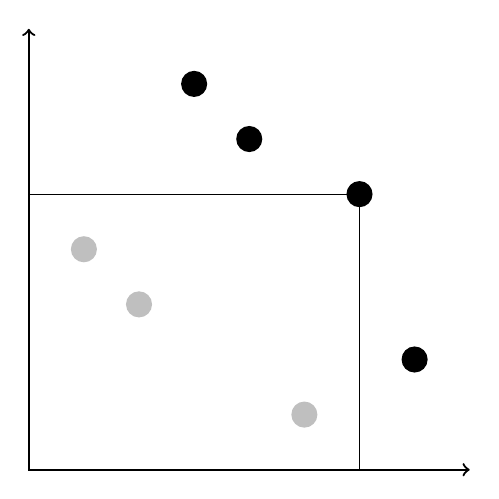
\begin{tikzpicture}[scale = .7, auto = center]
        \draw[thick, <->] (0,8) -- (0,0) -- (8,0);
        \node[circle, fill=lightgray] at (1,4) {};
        \node[circle, fill=lightgray] at (2,3) {};
        \node[circle, fill=black] at (3,7) {};
        \node[circle, fill=black] at (4,6) {};
        \node[circle, fill=lightgray] at (5,1) {};
        \node[circle, fill=black] at (6,5) {};
        \node[circle, fill=black] at (7,2) {};
        \draw (0,5) -- (6,5) -- (6,0);
      \end{tikzpicture}
    }

    \only<7>{ 
      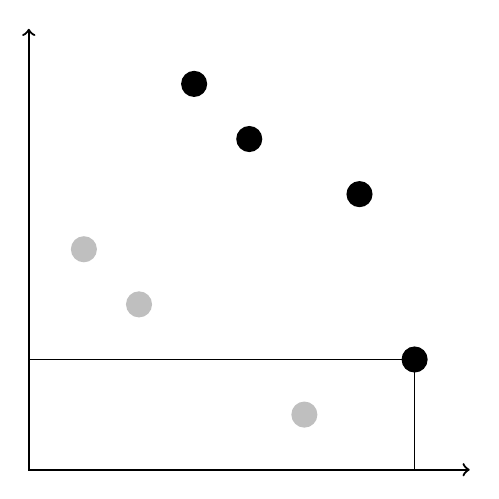
\begin{tikzpicture}[scale = .7, auto = center]
        \draw[thick, <->] (0,8) -- (0,0) -- (8,0);
        \node[circle, fill=lightgray] at (1,4) {};
        \node[circle, fill=lightgray] at (2,3) {};
        \node[circle, fill=black] at (3,7) {};
        \node[circle, fill=black] at (4,6) {};
        \node[circle, fill=lightgray] at (5,1) {};
        \node[circle, fill=black] at (6,5) {};
        \node[circle, fill=black] at (7,2) {};
        \draw (0,2) -- (7,2) -- (7,0);
      \end{tikzpicture}
    }

    \only<8>{ 
      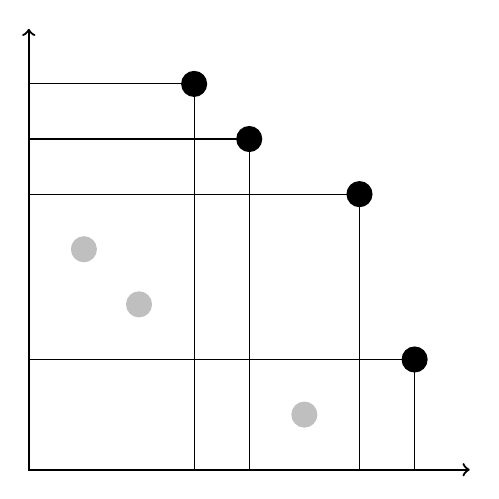
\begin{tikzpicture}[scale = .7, auto = center]
        \draw[thick, <->] (0,8) -- (0,0) -- (8,0);
        \node[circle, fill=lightgray] at (1,4) {};
        \node[circle, fill=lightgray] at (2,3) {};
        \node[circle, fill=black] at (3,7) {};
        \node[circle, fill=black] at (4,6) {};
        \node[circle, fill=lightgray] at (5,1) {};
        \node[circle, fill=black] at (6,5) {};
        \node[circle, fill=black] at (7,2) {};
        \draw (0,7) -- (3,7) -- (3,0);
        \draw (0,6) -- (4,6) -- (4,0);
        \draw (0,5) -- (6,5) -- (6,0);
        \draw (0,2) -- (7,2) -- (7,0);
      \end{tikzpicture}
    }

    \only<9>{ 
      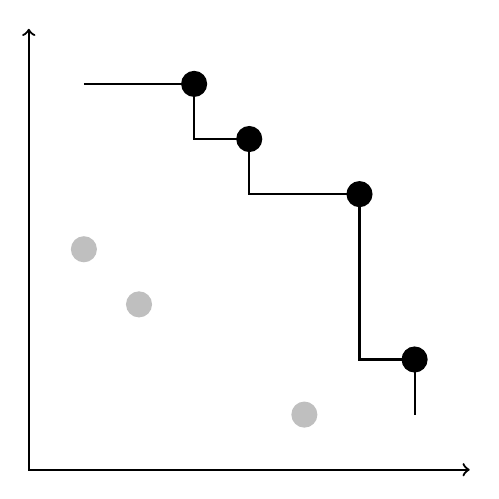
\begin{tikzpicture}[scale = .7, auto = center]
        \draw[thick, <->] (0,8) -- (0,0) -- (8,0);
        \node[circle, fill=lightgray] at (1,4) {};
        \node[circle, fill=lightgray] at (2,3) {};
        \node[circle, fill=black] at (3,7) {};
        \node[circle, fill=black] at (4,6) {};
        \node[circle, fill=lightgray] at (5,1) {};
        \node[circle, fill=black] at (6,5) {};
        \node[circle, fill=black] at (7,2) {};
        \draw[thick] (1,7) -- (3,7) -- (3,6) -- (4,6) --
                     (4,5) -- (6,5) -- (6,2) -- (7,2) --
                     (7,1);
      \end{tikzpicture}
    }

    \only<10>{ 
      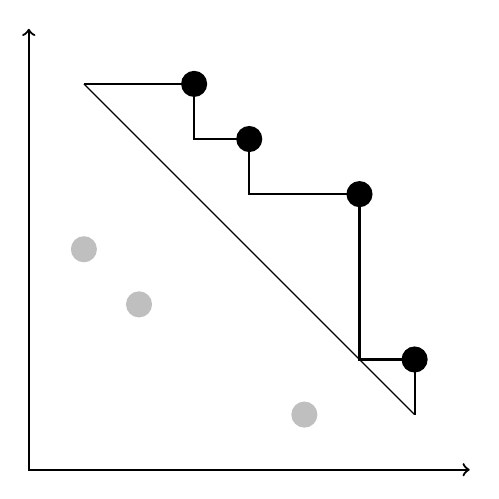
\begin{tikzpicture}[scale = .7, auto = center]
        \draw[thick, <->] (0,8) -- (0,0) -- (8,0);
        \node[circle, fill=lightgray] at (1,4) {};
        \node[circle, fill=lightgray] at (2,3) {};
        \node[circle, fill=black] at (3,7) {};
        \node[circle, fill=black] at (4,6) {};
        \node[circle, fill=lightgray] at (5,1) {};
        \node[circle, fill=black] at (6,5) {};
        \node[circle, fill=black] at (7,2) {};
        \draw[thick] (1,7) -- (3,7) -- (3,6) -- (4,6) --
                     (4,5) -- (6,5) -- (6,2) -- (7,2) --
                     (7,1);
        \draw (1,7) -- (7,1);
      \end{tikzpicture}
    }

    \only<11>{
      \begin{tikzpicture}[scale = .7, auto = center]
        \draw[thick, color =  white] (0,8) -- (0,0) -- (8,0);
        \draw[thick] (0,2) -- (2,4) -- (3,3) -- (4,4) --
                     (5,3) -- (7,5) -- (10,2) -- (11,3) --
                     (12,2);
        \draw (0,2) -- (12,2);
      \end{tikzpicture}
    }

    \only<12,13>{
      \begin{tikzpicture}[scale = .7, auto = center]
        \draw[thick, color =  white] (0,8) -- (0,0) -- (8,0);
        \draw[thick] (0,2) -- (2,4) -- (3,3) -- (4,4) --
                     (5,3) -- (7,5) -- (10,2) -- (11,3) --
                     (12,2);
        \draw (0,2) -- (12,2);
        
        \node at (2,5) {2};
        \node at (4,5) {2};
        \node at (7,6) {3};
        \node at (11,4) {1};
      \end{tikzpicture}
    }

    \only<14>{
      \begin{tikzpicture}[scale = .7, auto = center]
        \draw[thick, color =  white] (0,8) -- (0,0) -- (8,0);
        \draw[thick] (0,2) -- (2,4) -- (3,3) -- (4,4) --
                     (5,3) -- (7,5) -- (10,2) -- (11,3) --
                     (12,2);
        \draw (0,2) -- (12,2);
        \draw (1,3) -- (9,3);
        \draw (10,1) -- (10,5);
      \end{tikzpicture}
    }

    \only<15>{
      \vspace{.1pc}

      \begin{tikzpicture}[scale = .7, auto = center]
        \draw[thick, color =  white] (0,8) -- (0,0) -- (8,0);
        \draw[thick] (0,2) -- (2,4) -- (3,3) -- (4,4) --
                     (5,3) -- (7,5) -- (10,2) -- (11,3) --
                     (12,2);
        \draw (0,2) -- (12,2);
        \draw (1,3) -- (9,3);
        \draw (10,1) -- (10,5);

        \node at (5,5) {$uH(x,u)$};
        \node at (11,5) {$H(x,u)$};
      \end{tikzpicture}
    }

  \end{figure}


    $$ \only<4-13>{\num_{213}(p)}  \uncover<4-13>{ = \binom{2}{2}}
    \only<5-13>{ + \binom{2}{2}} \only<6-13>{ + \binom{3}{2}}
    \only<7-13>{ + \binom{1}{2}} \only<8-13>{ = 5  }
    \only<14->{H(x,u) = } 
    \only<15->{ux (H(x,u) + 1) C(x) + xC(x) H(x,u)}  
    $$ 

\end{frame}


\begin{frame}{Sketch of proof} 
  
  Let $h_{n,k}$ denote the total number of peaks at height
  $k$ in all Dyck paths of semilength $n$. 
  Let $H(x,u) = \sum_{n,k \geq 0} h_{n,k} x^n u^k$. 
  
  \vspace{2pc}

  $$ \begin{aligned}
  H(x,u) &= \frac{uxC(x)}{1-uxC(x)-xC(x)}. \\
  \pause
   A^*(x) &= \sum_{n \geq 0} \binom{k}{2} h_{n-1,k} x^n \\
  \pause
    A^*(x) &= \frac{\left. x \partial_u ^2 H(x)\right|_{u=1}}{2} \\
         \pause
         &= \frac{x^3C(x)}{(1-4x)^{3/2}} \\ 
         \pause
         &= x^3 + 7x^4 + 38x^5 + 187^6 + \ldots
      \end{aligned} $$
    \pause
    \begin{flushright} $ \qed $ \end{flushright}

\end{frame}


\begin{frame}{Corollaries}
  \pause
  \begin{block}{Corollary}
    $$ \num_{231}(\Av_n 123) = \num_{231}(\Av_n 132)$$
  \end{block}
\end{frame}


\begin{frame}{Corollaries}

    $$ A(x) = \frac{x-1}{2(1-4x)} - \frac{3x-1}{2(1-4x)^{3/2}}$$

    $$B(x) = \frac{3x-1}{(1-4x)^{2}} - \frac{4x^2 - 5x +
    1}{(1-4x)^{5/2}}$$

    $$ D(x) =   \frac{ 8x^3 - 20x^2 + 8x - 1}{(1-4x)^{2}} 
      - \frac{36x^3 - 34x^2 + 10x - 1}{(1-4x)^{5/2}} $$ 

\end{frame}




\begin{frame}{Corollaries}

  $$ a_n = \frac{n+2}{4} \binom{2n}{n} - 3 \cdot 2^{2n-3} $$\\[.5pc]
  $$ b_n = (2n-1) \binom{2n-3}{n-2} - (2n+1)\binom{2n-1}{n-1} + 
     (n+4) \cdot 2^{2n-3}$$\\[.5pc]
  $$ \begin{aligned} d_n 
      &= \frac{1}{6} \binom{2n+5}{n+1} \binom{n+4}{2} 
      - \frac{5}{3} \binom{2n+3}{n} \binom{n+3}{2} \\
      &+ \frac{17}{3} \binom{2n+1}{n-1} \binom{n+2}{2} 
      - 6\binom{2n-1}{n-2} \binom{n+1}{2} - (n+1) \cdot 4^{n-1}.
    \end{aligned}
  .$$

\end{frame}


\begin{frame}{Corollaries}

  $$ a_n \sim \sqrt{\frac{n}{\pi}} 4^n$$
  $$ b_n \sim \frac{n}{2} 4^n $$
  $$ d_n \sim \frac{8}{3} \sqrt{\frac{n^3}{\pi}} 4^n. $$

\end{frame}


\begin{frame}{Larger patterns}
  \pause
  \begin{block}{Lemma}
    $$ \begin{array}{ccccc}
      2A(x) & + 2B(x) & + D(x) & = & \frac{x^3}{6} (C(x))'''\\
      4A(x) & + 2B(x) & & =&  x^3(J(x)/x^2)' 
      \end{array} $$
  \end{block}
  \pause
  \begin{block}{Theorem}
    For large enough $n$, the descending pattern of length $k$ occurs
    more often than any other length $k$ pattern in $\Avn$. 
  \end{block}
\end{frame}

\begin{frame}{Further Directions}
  \pause
  \begin{block}{Question}
    Are there any other `surprising' symmetries across or within permutation
    classes?
  \end{block}

  \pause

  \begin{block}{Note}
    The increasing and decreasing patterns are not always the extremes of the
    class: $\num_{123} (\Av 2413) = \num_{321} (\Av 2413) $ 
  \end{block}
  \pause

  \vspace{1pc}

  \begin{center}
  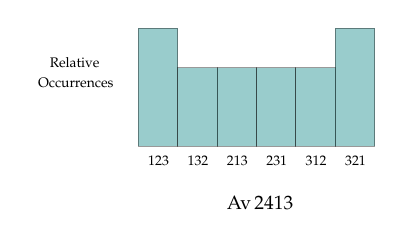
\begin{tikzpicture}
  [scale = .5]
  \foreach \x/\y in {0/3,1/2,2/2,3/2,4/2,5/3}{
    \draw[color = black, fill = teal, opacity = .4] (\x,0) rectangle (\x+1,\y);
  }
  \draw (0, 0) node[anchor=north west] {\tiny $123$};
  \draw (1, 0) node[anchor=north west] {\tiny $132$};
  \draw (2, 0) node[anchor=north west] {\tiny $213$};
  \draw (3, 0) node[anchor=north west] {\tiny $231$};
  \draw (4, 0) node[anchor=north west] {\tiny $312$};
  \draw (5, 0) node[anchor=north west] {\tiny $321$};
  \draw (2,-1) node[anchor=north west] {\scriptsize $\Av 2413$};
  \draw (-2.5, 2.5) node[anchor=north west] {\tiny Relative};
  \draw (-2.8, 2) node[anchor=north west] {\tiny Occurrences};
  \end{tikzpicture} 
  \end{center}
\end{frame}

\newgeometry{margin=0mm}
\begin{frame} \frametitle{\hspace{28pt}The Pattern Poset} \pause
  \begin{center}
    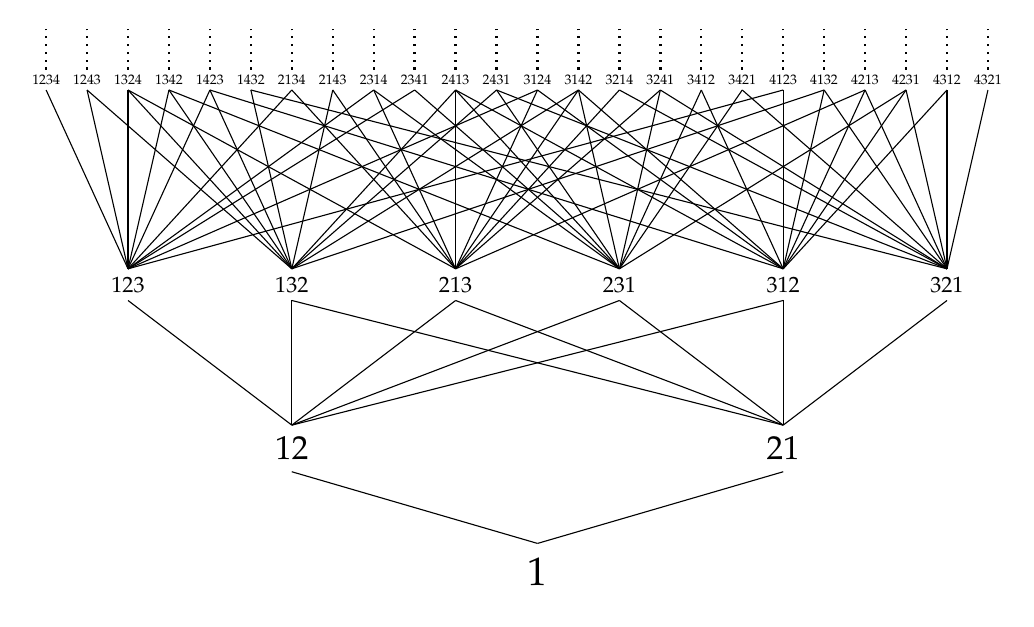
\begin{tikzpicture}[
    every node/.style={},
    scale=.52]
      {\Large
      \node (1) at (12,0) {1};
      }

      \pause

      {\large
      \node (12) at (6,3) {12};
      \node (21) at (18,3) {21};
      }

      \pause

      \draw (12.south)-- (1.north);
      \draw (21.south) -- (1.north);

      \pause

      {\footnotesize
      \node (123) at (2 ,7) {123};
      \node (132) at (6 ,7) {132};
      \node (213) at (10,7) {213};
      \node (231) at (14,7) {231};
      \node (312) at (18,7) {312};
      \node (321) at (22,7) {321};
      }

      \pause

      \draw (123.south) -- (12.north);
      \draw (132.south) -- (12.north);
      \draw (213.south) -- (12.north);
      \draw (231.south) -- (12.north);
      \draw (312.south) -- (12.north);
      
      \draw (132.south) -- (21.north);
      \draw (213.south) -- (21.north);
      \draw (231.south) -- (21.north);
      \draw (312.south) -- (21.north);
      \draw (321.south) -- (21.north);

      \pause
      
      {\tiny
      \node (1234) at (0 ,12) {1234};
      \node (1243) at (1 ,12) {1243};
      \node (1324) at (2 ,12) {1324};
      \node (1342) at (3 ,12) {1342};
      \node (1423) at (4 ,12) {1423};
      \node (1432) at (5 ,12) {1432};

      \node (2134) at (6 ,12) {2134};
      \node (2143) at (7 ,12) {2143};
      \node (2314) at (8 ,12) {2314};
      \node (2341) at (9 ,12) {2341};
      \node (2413) at (10,12) {2413};
      \node (2431) at (11,12) {2431};

      \node (3124) at (12,12) {3124};
      \node (3142) at (13,12) {3142};
      \node (3214) at (14,12) {3214};
      \node (3241) at (15,12) {3241};
      \node (3412) at (16,12) {3412};
      \node (3421) at (17,12) {3421};

      \node (4123) at (18,12) {4123};
      \node (4132) at (19,12) {4132};
      \node (4213) at (20,12) {4213};
      \node (4231) at (21,12) {4231};
      \node (4312) at (22,12) {4312};
      \node (4321) at (23,12) {4321};
      }

      \pause 

      % 123
      \foreach \p in {1234, 1243, 1324, 1342, 1423, 2134, 2314, 2341, 3124, 4123}
        \draw (\p.south) -- (123.north);
      % 132
      \foreach \p in {1243, 1324, 1342, 1423, 1432, 2143, 2413, 2431, 3142, 4132}
        \draw (\p.south) -- (132.north);
      % 213
      \foreach \p in {1324, 2134, 2143, 2314, 2413, 3124, 3142, 3214, 3241, 4213}
        \draw (\p.south) -- (213.north);
      % 231
      \foreach \p in {1342, 2314, 2341, 2413, 2431, 3142, 3241, 3412, 3421, 4231}
        \draw (\p.south) -- (231.north);
      % 312
      \foreach \p in {1423, 2413, 3124, 3142, 3412, 4123, 4132, 4213, 4231, 4312}
        \draw (\p.south) -- (312.north);
      % 321
      \foreach \p in {4321, 3421, 4231, 2431, 3241, 4312, 4132, 1432, 4213, 3214}
        \draw (\p.south) -- (321.north);

      \pause 

      \foreach \p in {1234, 1243, 1324, 1342, 1423, 1432,
                      2134, 2143, 2314, 2341, 2413, 2431,
                      3124, 3142, 3214, 3241, 3412, 3421,
                      4123, 4132, 4213, 4231, 4312, 4321}
        \draw[dotted, line width=.3mm] (\p.north) -- ++(0,1);

    \end{tikzpicture}
  \end{center}
\end{frame}
\restoregeometry

\end{document}
